\chapter{Praktische Umsetzung}
\label{cha:praxis}

\section{Situationsbeschreibung}
\label{sec:situation}

Die bestehende Situation spielt für die spätere Umsetzung eine große Rolle und muss somit im näheren betrachtet werden.
Zu Beginn des Projektes wurden bereits diverse Systeme zur Überwachung des Netzwerkes eingesetzt. Hierunter fällt die Überwachung der Stati der einzelnen Netzwerk Geräte, im speziellen die Switchs und Router, welche über das Programm “OpenView” von HP erfasst werden. Über dieses Programm können ebenfalls Server und deren Dienste erfasst werden. Diese Funktion wird jedoch aktuell nicht mehr mit Daten gepflegt, da hier ein Transfer zu einem anderen System stattfindet, aufgrund der Tatsache, dass die Lizenz von OpenView ausgelaufen ist. Im Moment dient das OpenView System bei Pirelli Deutschland GmbH dazu, dass eine automatische Übersicht über die Relationen zwischen den Switchs und Routern erstellt werden kann.\\
Für die Überwachung spezieller Hosts (in der Praxis meist Server) und Diensten, kommt ein weiteres System zum Einsatz, welches eine Open Source Software ist und ein hohes Maß an Flexibilität und Modularität bietet. Dieses “Nagios” gennante Programm ermöglicht es diverse Dienste im Netzwerk auf vorgegebenen Hosts abzufragen und anschließend diese zu visualisieren. Zusätzlich können verschiedene Warn- und Fehlerlevels für einen Service definiert werden, die im Falle einer Störung Warnungen an vordefinierte Personen verschicken.\\
Dieses System ist somit hauptsächlich für die Überwachung der Dienste zuständig.\\
Zur Untersuchung von Netzwerk-Traffic zwischen verschiedener Netzwerke kommt das System MRTG zum Einsatz welches hauptsächlich für das Anzeigen des Netzwerktraffics auf Routern ausgelegt ist.
Dieses wird im Unternehmen hauptsächlich zum Erfassen der Bandbreitennutzung der Router bzw. der WAN-Verbindungen zu überprüfen.
Dies ist vor allem wichtig um den aktuellen Traffic zwischen den einzelnen Standorten in Deutschland im Überblick zu behalten.\\
Abschließend gibt es noch ein System von Cisco, mit dem Namen “CiscoWorks” welches dazu dient mit einem speziellen Programmteil die Hosts an den jeweiligen Switchs zu erkennen und zu identifizieren.
Hier werden nicht nur simple Zuordnungen zwischen Mac-Adresse des Hosts und des Switchs, bzw. des Port des Switches hergestellt.
Sondern umfangreiche Informationen gesammelt, z.B. über die Geschwindigkeit des Anschlusses, die IP und, sofern vorhanden, der DNS-Hostname des Gerätes.
Hinzukommen diverse Details, wie der Gerätetyp, welcher einem die Möglichkeit gibt, zu erkennen ob es sich hierbei um ein Switch oder Router handelt.\\
Da es bei diesem System notwendig ist, regelmäßig die Lizenz zu verlängern um auch weiterhin die neusten Router und Switches zu unterstützen, ist hier eine gewisse Abhängigkeit gegeben.
Weil von CiscoWorks selbst nur ein kleiner Teil genutzt wird und somit die Lizenzkosten unverhältnismäßig zur Nutzung sind, wurde entschieden diese in Zukunft zu ersetzen.\\

Die Überwachung des Netzwerks lässt sich bei näherer Betrachtung in folgende Punkte unterteilen:\\
Überwachung von Diensten/Servern\\
Überwachung des Netzwerkverkehrs\\
Darstellung und Überwachung des Netzwerkequipments\\
Überwachung von einzelnen Hosts im Netzwerk\\

Das Netzwerk selbst bei Pirelli Deutschland GmbH ist in verschiedenen Hierachie-Ebenen konzepiert.
In der untersten Ebene stehen die Switchs an denen die Hosts angeschlossen sind. Diese Ebene wird als Access-Layer bezeichnet.
Über dieser Ebene wiederrum befinden sich der Distribution-Layer. In diesem sind Switchs zu finden, welche alle Access-Layer Switchs verbinden und als Schnittstelle zu den Layer 3 Switchen, den sogenanntne Core-Switches, dienen.
Die Core-Switches können zusätzlich anhand von OSI-Layer-3 Informationen Forwarding betreiben.
Die komplette Anordnung ist in Abbildung X zu sehen.


\begin{figure}[H]
\centering
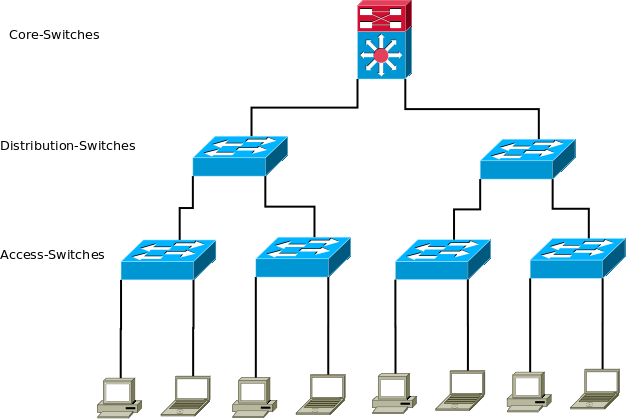
\includegraphics[width=0.9\textwidth]{network_ex1.png}
%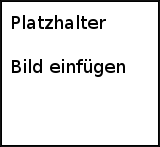
\includegraphics[width=0.8\textwidth]{000.PNG}
\caption{Netzwerkarchitektur PD}
\label{fig:show_s1_s2_p1_n1}
\end{figure}

\section{Anforderungsdefinition}
\label{sec:anfdef}

Um das bestehende System ersetzen zu können muss zunächst untersucht werden, welche der bereits vorhandenen Funktionen im aktuell verwendeten System genutzt werden und welche in Zukunft benötigt werden.\\
Im Anschluss dieser Untersuchung müssen auch weitere potentielle Aufgaben berücksichtigt werden um eine Erweiterbarkeit des Systems zu garantieren.
Damit das neue System allen Anforderungen gerecht wird empfiehlt es sich zunächst sich mit den Personen zusammen zu setzten, die das bestehende Programm zur Zeit nutzen.\\
Hierbei wird nicht nur auf die aktuelle Nutzung eingegangen, sondern auch diese kritisch hinterfragt, ob eventuelle Anforderungen bereits von anderen Systemen erfüllt werden.
Durch Gespräche mit den zuständigen Mitarbeitern wurden diverse Anforderungen erörtert.\\
Als wichtigster Punkt ist die Erkennung der Hosts, sowie der zugehörigen Ports an den Switchs zu sehen.
Diese ist notwendig um den Ort eines Hosts im Netzwerk festzustellen. Praktische Anwendung hat dies, wenn zum Beispiel ein Host aufgefunden werden muss, wenn der zugehörige Mietschein des Computers ausläuft und dieser zurückgegeben werden muss.
Hier ist es nicht selten der Fall, dass der Computer mit seinem dazugehörigen Besitzer bereits die damalige Abteilung verlassen hat und dieser somit nicht mehr auffindbar ist.
Eine weiterere Anwendungsmöglichkeit ist, dass der Helpdesk wissen möchte, wenn es Probleme mit einem Computer gibt, ob die Netzwerk-Hardware bis zum Host einwandfrei funktioniert. Hierfür musss man nicht nur wissen, an welchem Ort der Host sich befindet, sondern auch die dazugehörigen Ports.
Da die Ports als auch die Switchs ausgelesen werden, kann man somit zeitnah eine Rückmeldung geben, dass der Switch, so wie dessen Port einwandfrei funktionieren, oder falls dies nicht der Fall ist, den Fehler besser lokalisieren. Somit ist selbst bei keinerlei Kenntnis des Hosts außer der DNS oder der IP eine direkte Lokalisierung und Bewertung des Status möglich.\\
Ein weiterer wichtiger Aspekt ist die Möglichkeit genau herauszufinden, welche Hosts hinter einem Port angeschlossen sind.
In der Praxis ist dies wichtig, da es vorkommen kann, dass unerwünschte Netzwerkgeräte angeschlossen wurden.
Normalerweise befinden sich im Unternehmen an einem Port eines Switches der untersten Ebene maximal zwei Hosts. Der Großteil der Ports hat nur einen Host zum Beispiel den Computer eines Mitarbeiters oder ein Netzwerkgerät. In einem Teil der Fälle ist dieser Computer nicht direkt an den Port des Switches angeschlossen, sondern wird über den Port eines VOIP-Telefons durchgeschleift, welches dann an den Switch angeschossen ist.
In diesem Fall sind auf dem Port zwei Hosts zu sehen.
Dies ist der Soll Zustand. Jedoch kann es vorkommen, das Mitarbeiter im Werk ohne Erlaubnis fremde Netzwerkgeräte anbringen, sei es ein Hub, ein eigener WLAN-Router oder andere Geräte. Da diese Geräte die Sicherheit des Netzwerkes beeinflussen, müssen diese identifiziert und gleichzeitig lokalisiert werden können um eine Entfernung zu ermöglichen.
Hinzu kommt der Punkt einer möglichen Historie, wann welcher Host an welchem Port bzw. Switch angeschlossen war. Hierbei soll erkennbar sein, an welchem Port der Host war, jedoch ist es nicht notwendig zu wissen wie oft dieser dort angeschlossen war. Beispielsweise gibt es den Switch S1 und S2. Zu Beginn ist der Host, in diesem Falle ein Notebook N1, an einen Port P1 an S1 angeschlossen.\\
Nun wechselt N1 zu P1 an S2.
Hierfür soll nun ein Eintrag in der Datenbank erzeugt werden. Wenn N1 jetzt wieder von P1 auf S2 auf P1 auf S1 wechselt, so soll kein neuer Eintrag entstehen, sondern nur der bereits existierende aktualisiert werden. Wechselt N1 jedoch von P1 auf S1 zu P2 auf S1, so soll ebenfalls ein neuer Eintrag erzeugt werden.\\

\begin{figure}[H]
\centering
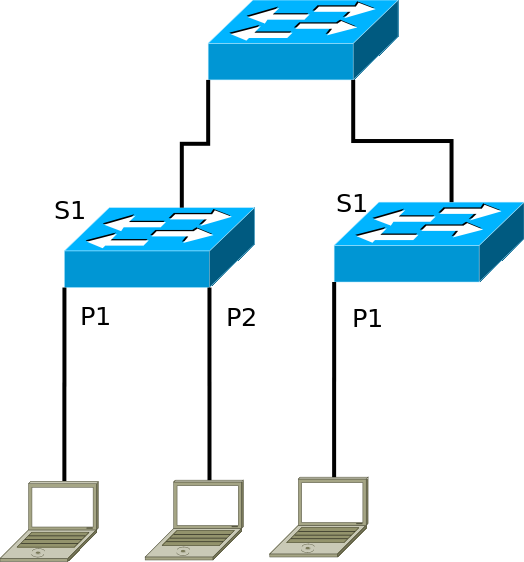
\includegraphics[width=0.4\textwidth]{network_ex2.png}
%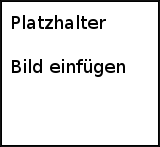
\includegraphics[width=0.5\textwidth]{000.PNG}
\caption{Grafik mit S1+S2 sowie jeweils P1 und N1}
\label{fig:show_s1_s2_p1_n1}
\end{figure}


Für das Auslesen der Switches soll das Netzwerkprotokoll SNMP verwendet werden, da eine Abfrage per Telnet die Switches stark belastet und somit es passieren kann das der Betrieb eingeschränkt wird. Hinzu kommt, dass ein Auslesen per Telnet sehr langsam ist und die Ausgabe selbst nicht standardisiert ist und somit sehr viele Einzelfälle behandelt werden müssten.\\
Im Hinblick auf die Geschwindigkeit des Auslese-Prozesses wurde vorausgesetzt, dass das Sammeln der Daten mindestens vier mal am Tag möglich sein muss und sofern möglich sollte eine Auslesezeit unter 60 Minuten angestrebt werden, da es sich hierbei um einen alten Wert handelt, welcher bei früheren Auslesevorgängen erreicht wurde.\\

Eine weitere Anforderung die als optional angesehen wird, ist die Möglichkeit die Verbindungen zwischen den Switches und Routern zu erfassen. Das heißt, es soll eine Topologie anhand der Daten erstellt werden können.\\
Zu den optionalen Anforderungen gehört die Möglichkeit einer Benutzerzuordnung zu den jeweiligen Hosts. Die Zuordnung soll über das bestehende Active Directory passieren und somit die Möglichkeit bieten den entsprechenden Nutzer direkt anrufen zu können bei Problemen.\\
Kombiniert man diese Anforderungen so bildet sich eine weitere Anwendungsmöglichkeit und zwar kann es in der Praxis vor kommen, dass ein Switch gewechselt und somit abgeschaltet werden muss. Hierfür kann man nun im Voraus kontrollieren, welche Hosts an diesen angeschlossen sind und die dementsprechenden Nutzer im Voraus zu informieren.\\

Neben den Anforderungen zu den Anwendungsmöglichkeiten wurden auch Anforderungen an das Programm selbst gestellt.
Zu diesen gehört die Betriebsystemunabhängigkeit.
Das Programm muss sowohl auf dem Windows, als auch auf dem Linux Betriebsystem funktionieren. Sofern Interpretersprachen oder ähnliches verwendet werden, darf keine Versionsabhängigkeit bestehen, d.h. das Programm muss z.B. sowohl unter Java 1.6.0.10 als auch unter 1.6.0.33 funktionieren.\\
Als bestehende Datenbank wurde Oracle vorgegeben, da hierfür bereits Lizenzen existieren und diese bereits auf den entsprechenden Servern läuft und kein weiteres DBMS installiert und gepflegt werden muss.\\

\section{Anforderungsanalyse}
\label{sec:anfanalyse}

Um die Anforderungen bewerten zu können, muss man sich zunächst mit den Technologien vertraut machen und die technischen Möglichkeiten mit den Anforderungen abgleichen.\\
Zunächst einmal muss untersucht werden, ob die im Unternehmen befindlichen Switches auch das SNMP-Protokoll soweit unterstützen, um das Auslesen zu ermöglichen.
Dies wurde überprüft und bei vereinzelten Switches musste die Konfiguration angepasst werden, da hier teilweise SNMP deaktiviert oder nur für spezielle Hosts zugelassen war.\\
Im nächsten Schritt galt es zu Überprüfen, ob die benötigten Informationen per SNMP überhaupt abfragtbar sind. Problematisch hierbei ist vor allem, dass Hersteller zwar eigene MIBs bei SNMP verwenden, über diese lassen sich jedoch nicht die gleichen Informationen abfragen wie über die proprietären Protokolle der Hersteller.
Bei der Überprüfung der Zuordnung zwischen Mac-Adresse der angeschlossenen Ports wurde festgestellt, dass diese zwar möglich ist, aber eine sehr spezielle Vorgehensweise vorrausetzt [vgl. SNMP Cisco PDF].\\
Problematisch ist vorallem die genaue Zuordnung der Hosts an den korrekten Switch. So kann es sein, dass die Mac-Adresse eines Hosts sowohl auf einem Access-Switch als auch auf einem Distribution-Switch zu finden ist. Hierfür muss eine eindeutige Identifizierung stattfinden, welcher Switch welche Hierarchie Ebene angehört. Diese Informationen müssten manuell gepflegt werden oder anhand einer automatischen Hierachie Erkennung erhalten werden.\\
Die Anforderung alle Hosts hinter einem Port zu finden stellt kein Problem dar, da dies von allen Switches per SNMP unterstützt wird. \\
Eine Historie die es ermöglicht nur neue Kombinationen aus Mac des Hosts und zugehöriger Port als neuen Eintrag zu sehen ist ohne Probleme möglich und kann durch die demensptrechende Erstellung der Datenbank sichergestellt werden.\\
Aussagen über die Geschwindigkeit können leider im Voraus nicht getroffen werden, jedoch ist anzunehmen, dass die Geschwindigkeit über der des manuellen Auslesens per Telnet liegen muss, da SNMP nicht Verbindungsorientiert ist und somit die Endgeräte weniger belastet werden und der Overhead reduziert ist. Genauere Aussagen über die Geschwindigkeit lassen sich erst durch Benchmarks machen, welche in Kapitel [Kapitel X] durchgeführt werden.\\
Um mögliche Verbindungen zwischen den Switches und Routern zu Erfassen muss es möglich sein auf einem Port einen Switch zu identifizieren, was per SNMP in Verbindung mit STP und CDP möglich ist.\\
Eine Zuordnung der einzelnen Nutzer lässt sich über das Active Directiry per LDAP bewerkstelligen, hierfür muss aber ein spezieller Benutzer eingerichtet werden, der vollständige Leserechte für alle Hosts im Netzwerk besitzt.\\
Die Betriebsystem Unabhängigkeit ist mit einer Vielzahl von Interpreter-Sprachen (Perl, Phyton, ...) oder einer Platform unabhänigen Sprache (Java, C Sharp/Mono) gegeben.\\
Da für alle gängigen Sprachen diverse Datenbank Anbindungen angeboten werden, gibt es bei der Wahl des DBMS auf Oracle keine Probleme.\\
Insgesamt betrachtet gibt es von der technischen Seite zwar gewisse Schwierigkeiten bei der Implementierung, diese hindern aber nicht eine Umsetzung des Projektes.\\

Ein weiterer wichtiger Punkt sind auch die Ressourcen, da für die komplette Implementierung nur 11 Wochen zur Verfügung stehen. Für eine Implementierung eines Systems mit diesem Umfang und einer ausreichenden Testphase bei nur einem Entwickler ist dies ein zu geringer Zeitraum. Da vor der Implementierung und den Tests zuerst einmal der Entwurf und gewisse Design Entscheidungen stehen müssen, wird es hier zu Engpässen kommen, welche nur durch Kompromisse im Hinblick auf die Implementierung und den Tests gelöst werden können.\\
Da ein Großteil der Zeit für das Auslesen der Daten aufgebracht werden muss, wird die Zeit für die Umsetzung der Weboberfläche relativ kurz geraten. Hier muss dann im Laufe des Projektes abgewägt werden zwischen einzelnen Punkten.\\

Im Hinblick auf die Kosten entstehen bei der Umsetzung keine weitere Kosten bzw. bei der Wahl eines existierenden Open Source-Systems. Ziel des Projektes ist das bestehende kommerzielle Produkt zu ersetzen und somit eine monitäre Einsparung, aber auch der Anforderung einer gewissen Modularität gerecht zu werden.\\

\section{Betrachtung bereits existierender Lösungen}
\label{sec:exitloesungen}

Betrachtet man die bereits existierenden Lösungen zum Überwachen von Switches und Hosts, so lassen sich einige Produkte finden, die kommerzieller Natur als auch Open Source sind.
Bei HP Openview handelt es sich um eine kommerziell Lösung von HP, die dazu dient eine komplette Netzwerk und Systemmanagement-Lösung anzubieten. Diese Software-Umgebung besteht nicht nur aus HP eigenen Modulen sondern auch von verschiedenen Fremdherstellern.
Die wichtigste Komponente des HP Openview für die Netzwerküberwachung stellt der sogenannte ‘HP OpenView Network Node Manager’ dar. Dieser ermöglichst es neben dem Überblick über die Netzwergeräte und deren Stati zusätzlich detailierte Informationen zu den einzelnen Geräten anzuzeigen. Es bietet zusätzlich Histogramme z.B. für den aktuellen Durchsatz an.
Ebenso bietet sich die Möglichkeit einer Art Übersichtskarte die automatisch anhand der vorhandenden Netzwerkgeräte generiert wird. Die notwendigen Informationen hierfür werden per SNMP und CDP ausgelesen. Zusätzlich wird zur Statusüberprüfung auf Funktionen wie ein Ping zurückgegriffen\\
Eine weiteres kommerzielles System ist CiscoWorks von Cisco. Dieses bietet untere anderem ein spezielles Usertracking-Modul, welches einem ermöglicht alle Hosts in einem Netzwerk zu identifizieren, aber auch die dazugehörigen Switches, an die jeweils die Geräte angeschlossen sind anzuzeigen. Diese Informationen können teilweise auch per CDP (Cisco Discovery Protokoll) ausgelesen werden. Über die per CDP bereitgestellten Daten wird auch ein automatisches sequentielles Auslesen aller Switches im Netzwerk ermöglicht, ohne zuvor diese zu kennen (Zugriffsrechte werden trotzdem benötigt).\\
Das Open Source Programm Nagios dient vor allem zum Überwachen von verschiedenen Geräten im Netzwerk, sowie deren Dienste. Hierbei arbeitet es ebenfalls per SNMP. Es ist aber nicht auf dieses allein angewiesen. Sofern eingerichtet kann auch per einfach TCP oder UDP Dienste überprüft werden. Es können aber auch Remote Skripts per SSH aufgerufen werden.
Jedoch ist hierbei zu Beachten das Nagios nur das Überwachen von bekannten und zuvor konfigurierten Hosts und Diensten unterstützt und somit für die gewünschte Anforderung nicht in Frage kommt.\\
Ein System  was die Anforderungen teilweise erfüllt ist Tirtih. Dieses Programm wird vom Fraunhofer Institut eingesetzt im Kompetenzzentrum Netzwerkmanagement und ist Open Source. Es unterstützt das Auslesen von diversen Cisco Switches sowie deren jeweiligen Hosts.
Zusätzlich ließt Tirtih eine Großzahl an Infromationen über die Switches sowie das bestehende VLAN aus. Funktionen die Tirtih nicht bietet ist ein paralleles Auslesen der Switches und es verfügt auch nicht über eine Historie, wenn ein Port an einem Switch getauscht werden sollte.
\footnote{http://www.gambitcomm.com/site/products/mgmt\_apps/interopnet98.htm
http://www.fernuni-hagen.de/BWLPIT/LADV\_/PDF\_Dateien/Hinweise\_Anfertigung\_wiss\_Arbeiten.PDF}

\section{Entscheidung zur eigenen Herstellung}
\label{sec:decisionowncreating}

Vergleicht man alle aufgeführten Systeme so lässt sich feststellen, dass keine der genannten Lösungen den Anforderungen entspricht.
Zwar bietet Tirtih einen Teil der gewünschten Funktionen, jedoch müsste dies erst auf die speziellen Bedürfnisse angepasst werden, die das Unternehmen benötigt.
Aufgrund dieser Tatsache empfiehlt sich eine eigene Implementierung, da diese die Möglichkeit gibt besonderes auf die Anforderungen einzugehen und keine Einarbeitungszeit in eine fremde System-Architektur notwendig macht.
Selbstverständlich sind mit einer eigenen Implementierung gewisse Risiken verbunden, darunter auch der knappe Zeitrahmen.
In der Anforderungsanalyse wurden diese aber bereits abgewegt und eine Machbarkeit des Systems festgestellt.

\section{Entwurf}
\label{sec:Entwurf}


\subsection{Usecases}
\label{subsec:usecases}

Zu Beginn eines Projektes zur Entwicklung eines Systems müssen zuerst die Usecases identifiziert werden und die beteiligten Akteure.
Hierzu wird zu Beginn überlegt welche Personen Zugang zum System haben und welche Aufgaben diese am System erfüllen werden.
Für den Entwurd wird nicht nur die Anforderungsdefinition zu Rate gezogen, sondern bespricht die notwendigen Funktionalitäten, die das Programm später beinhalten soll, mit den Mitarbeitern selbst.
Dadurch kommen meist weitere Punkte auf die zuvor nicht angesprochen wurden, jedoch wichtig sind für den späteren Entwurf des Systems, sowie die Umsetzung.
In Abbildung X ist das Usecase-Diagramm für das System zu sehen.

\begin{figure}[H]
\centering
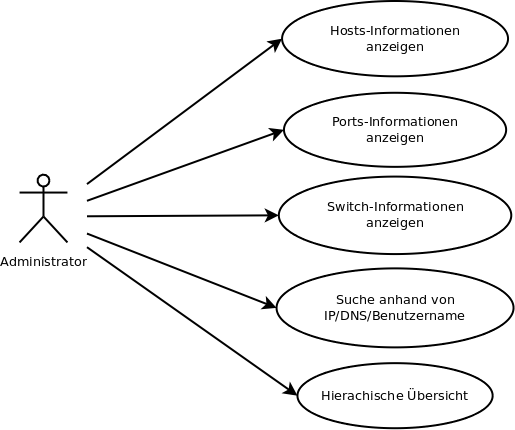
\includegraphics[width=0.8\textwidth]{UML_usecases.png}
\caption{Usecasediagramm}
\label{fig:usecase001}
\end{figure}

Zum einen ist festzustellen, dass es nur einen Akteur gibt. Das liegt daran, dass keine Einschränkung vorgesehen ist für die aktiven Nutzer des Systems. Bei der Implementierung wird jedoch eine mögliche spätere Einführung von verschiedenen Benutzerrechten bedacht und diese Funktionalität als Möglichkeit offen gelassen. Zur Einfachheit halber wird der Netzwerkdaminstrator im Laufe des Textes als Benutzer beschrieben.
Die erste Sicht die dem Nutzer zur Verfügung stehen muss ist eine Übersicht über alle Switches, hier muss neben der Switch IP auch der per SNMP ausgelesene Alias stehen, aber auch die vorhandene IOS-Version und die Seriennummer des Switchs.\\
In einer weiteren Sicht soll eine Übersicht auf die Ports eines Switches geben werden.
Neben der MAC-Adresse des Ports, so wie des Port Namens (z.B. Fa0/1) sind weitere Informationen sichtbar, unter Anderem der Status (Up/Down), Geschwindigkeit des Ports, sofern zugewiesen die VLAN ID, Duplexmodus, aber auch Informationen, ob es sich hierbei um ein Uplinkport handelt.
Zusätzlich wird eine Sicht benötigt, die Informationen über den angeschlossenen Host anzeigt. Hierunter fallen Informationen wie, MAC-Adresse, IP, DNS, sowie der zuletzt angemeldete Benutzer an einer Workstation. Zusätzlich sollen aber auch Informationen angezeigt werden, welche in Verbindung mit dem Port in Verbindung stehen. Diese werden im Zuge der Historie zusätzlich beim Host gespeichert. Sofer es sich um ein CDP-fähiges Gerät handeln sollte, werden diese zusätzliche Informationen ebenfalls angezeigt.
Neben den Sichten zu den Geräten wird es auch eine Übersicht der VLANs geben, welche es erlaubt eine Verbindnug herzustellen zwischen VLAN ID und des jeweiligen VLANs inkl. Name und  VTP-Domain.\\
Der Benutzer soll weiterhin auf jeder dieser Sichten eine Möglichkeit zur Suche eines Hosts/Switches haben, wie auch eine Option zur Sortierung der Einträge.
Neben diesen grundlegenden Funktionen wurde empfohlen zusätzlich eine Art hierarchische Übersicht zu ermöglichen. Das heißt, der Nutzer kann über die Switchübersicht einen Switch selektieren und erhält dann die Übersicht der dort verfügbaren Ports. Wählt er nun einen Port auf diesem Switch aus, so erhält er alle Hosts die an diesen Port angeschlossen sind. Sofern es sich dabei um mehrere Hosts handelt wählt er wiederum einen aus und landet schließlich in der Übersicht über den Host mit den detailierten Informationen.\\
Als optionaler Usecase wir das Anzeigen einer Art Dashboard gesehen. In diesem werden Informationen zusammen gefasst die nicht direkt erkenntlich über die einzelnene Sichten sind. Beispielsweise könnte man hier Dinge anzeigen lassen, wie z.B. Anzahl freier Ports, Switch mit den meisten freien Ports, TOP 5 Switches mit der höchsten Last, um nur eine Liste der potentiellen Informationen zu nennen.

\subsection{Klassendiagramme}
\label{subsec:classdiagrams}

Für die Umsetzung des Projektes wurde eine objektorientierte Programmiersprache gewählt, welche es erfordert Objekte von Klassen abzuleiten und die dementsprechenden Methoden dieser Klassen bzw. ihrer Objekte zu nutzen. Für die Umsetzung des Projektes wurde mit mehr als 25 Klassen gearbeitet um eine genügend genaue Abstrahierung und Modularität zu erreichen. Im Nachfolgenden wird auf die wichtigsten Klassen und deren beinhaltete Methoden eingegangen.\\
Das Ausleseprogramm wird über die Klasse \textit{SNMPTrack} initialisiert, welches auch der Name des Auslese-Skripts darstellt. Diese Klasse ist sozusagen die Hauptklasse von der alle weiteren Objekte erzeugt werden. Zu Beginn des Programms wie in Kapitel X zu sehen werden die Switches aus der XML-Datei ausgelesen. Um hier später die Möglichkeit zu geben die Informationen auch über eine andere Datenquelle einzulesen wurde eine spezielle Klasse \textit{SwitchListe} für das Einlesen der Switches geschaffen. Hierzu muss nur ein Objekt der Klasse erzeugt werden, welches mit dem Befehl \textit{getSwitchList} eine Liste der Switches zurückliefert. Diese kann dann im Hauptprogramm direkt weiterverwendet werden ohne dort die komplette XML-Logik hinterlegen zu müssen.\\
Über die Klasse \textit{SNMPConfig} können weitere Informationen ausgelesen werden die benötigt werden. So bietet diese Klasse Methoden an, welche das Debuglevel oder die Maximale Threadanzahl der Switchthreads zurückliefern. Durch diese Methoden können die Werte ohne Probleme von einer zentralen Stelle ausgelesen werden. Diese wiederum können aus einer beliebigen Datenquelle (XML, DB) kommen.\\
Die nächste wichtige Klasse ist die \textit{SNMPHandler} Klasse. Sie verwaltet alle SNMP Abfragen bzw. vereinfacht den Abruf eines SNMP Wertes oder im Falle eines SNMP-Walk der Abruf einer kompletten Liste. Hierzu muss der jeweiligen Methode nur das globale SNMP Objekt, welches aus der SNMP4J-API stammt, die benötigte OID, die IP auf dem der SNMP-Agent läuft, sowie der passende Community-String zum Auslesen übergeben werden. Je nach Methode liefert die entsprechende Methode dann ein String oder eine Array List mit Strings als Elemente zurück. Um die Rückgabe Werte des SNMP-Agents besser zu verstehen ist das folgende Beispiel aufgeführt:\\

<OID>!<Wert>\\

Mit reellen Daten gefüllt könnte ein Rückgabewert wiefolgt sein:\\

1.3.6.1.2.1.1.1!Linux WRT54G 2.4.20 2 Thu Dec 9\\


Durch das Zusammensetzten mit ! kann eine Verarbeitung stattfinden bzw. der Wert einfach abgelesen werden.\\
Um einen Switch auszulesen wird ein Objekt der Klasse \textit{SwitchWorkerThread} erzeugt und diesem das SNMP Objekt, die IP und die passende Read-Community übergeben. Dieses Objekt startet dann den intern einen Thread, welcher ein Objekt der Klasse Switch erzeugt und die entsprechenden Initialisierungs-Variablen übergibt. Im Anschluss wird die Methode refresh() des Switches aufgerufen, welches alle relevanten Informationen beginnt auszulesen und dabei wie in Kapitel X beschrieben vorgeht. In der refresh() Methode des Switches wiederum wird auf spezielle Klassen zurückgegriffen.\\
Eines dieser Klassen ist \textit{OIDL}, welche für OID-Library stehen soll und alle Aliase der OID die verwendet werden enthält. Diese Aliase sind per RFC spezifiziert und 1:1 abgebildet. So ergibt z.b. der Aufruf: \\

OIDL.sysDescr0\\

den String:\\

1.3.6.1.2.1.1.1.0\\

Dies ist vor allem notwendig um eine Übersicht über die verwendeten OID zu behalten bzw. erkennen zu können welcher Funktion hinter der OID steckt. Der nachfolgende Quellcode-Abschnitt verdeutlicht die Wichtigkeit der Text-Äquivalenz zu den IDs:\\

\begin{figure}[H]
\centering
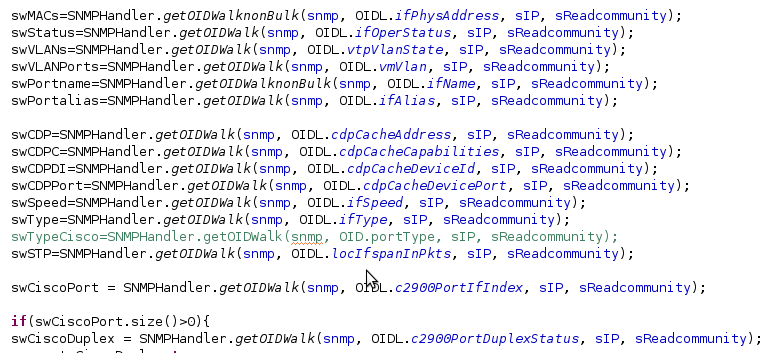
\includegraphics[width=0.8\textwidth]{code_example_OIDL.png}
\caption{Codebeispiel}
\label{fig:classdiagramcode}
\end{figure}

Im Programm selbst existieren jedoch auch Klassen die nicht nur zur Hilfe der eigenen Algorithmen Umsetzung dienen, sondern auch, welche externe Datenquellen anbinden.
Hierzu gehört die Klasse Nagios, welche per HTTP oder per MySQL Datenbank ermöglicht die Gruppenzuordnung der Switches auszulesen.
Hierzu gehört auch die Klasse LDAP, welche das Auslesen des Active Directories der Windows Domaine ermöglicht oder aber die Klasse DNSHelperClass, welche es ermöglicht auf mehreren DNS Servern einen DNS Namen anhand einer IP zu finden. Neben diesen Klassen gibt es aber auch speziell erstellte Klassen die es ermöglichen SQL-Befehle die keine Resultsets erwarten, dass heißt welche keinen Rückgabewert erwarten, in Stapel auszuführen.
Dies bedeutet, dass die Datenbank nicht jeden Befehl einzeln erhält sondern eine große Anzahl (>100 Stück) auf einmal und somit weniger Overhead für den Verbindungsaufbau entsteht.\\
Neben der Vielzahl von Klassen, welche zur Vereinfachung der Übersicht und Wartbarkeit dienen, gibt es trotzdem Objekte welche auch die Realtät abbilden. Dazu gehören die Klassen Switch (welche bereits beschrieben wurde), Ports, sowie Hosts. Diese bieten jeweils Methoden an, welche von sich selbst die passenden SQL-Befehle anhand der enthaltenen Daten generieren. Dies macht es vorallem einfach die Objekte zu serialisieren. Das heißt die Objekte im Programm wiederum abzubilden auf eine Textuale-Ebene, um sie in die Datenbank übertragen zu können.\\

\begin{figure}[H]
\centering
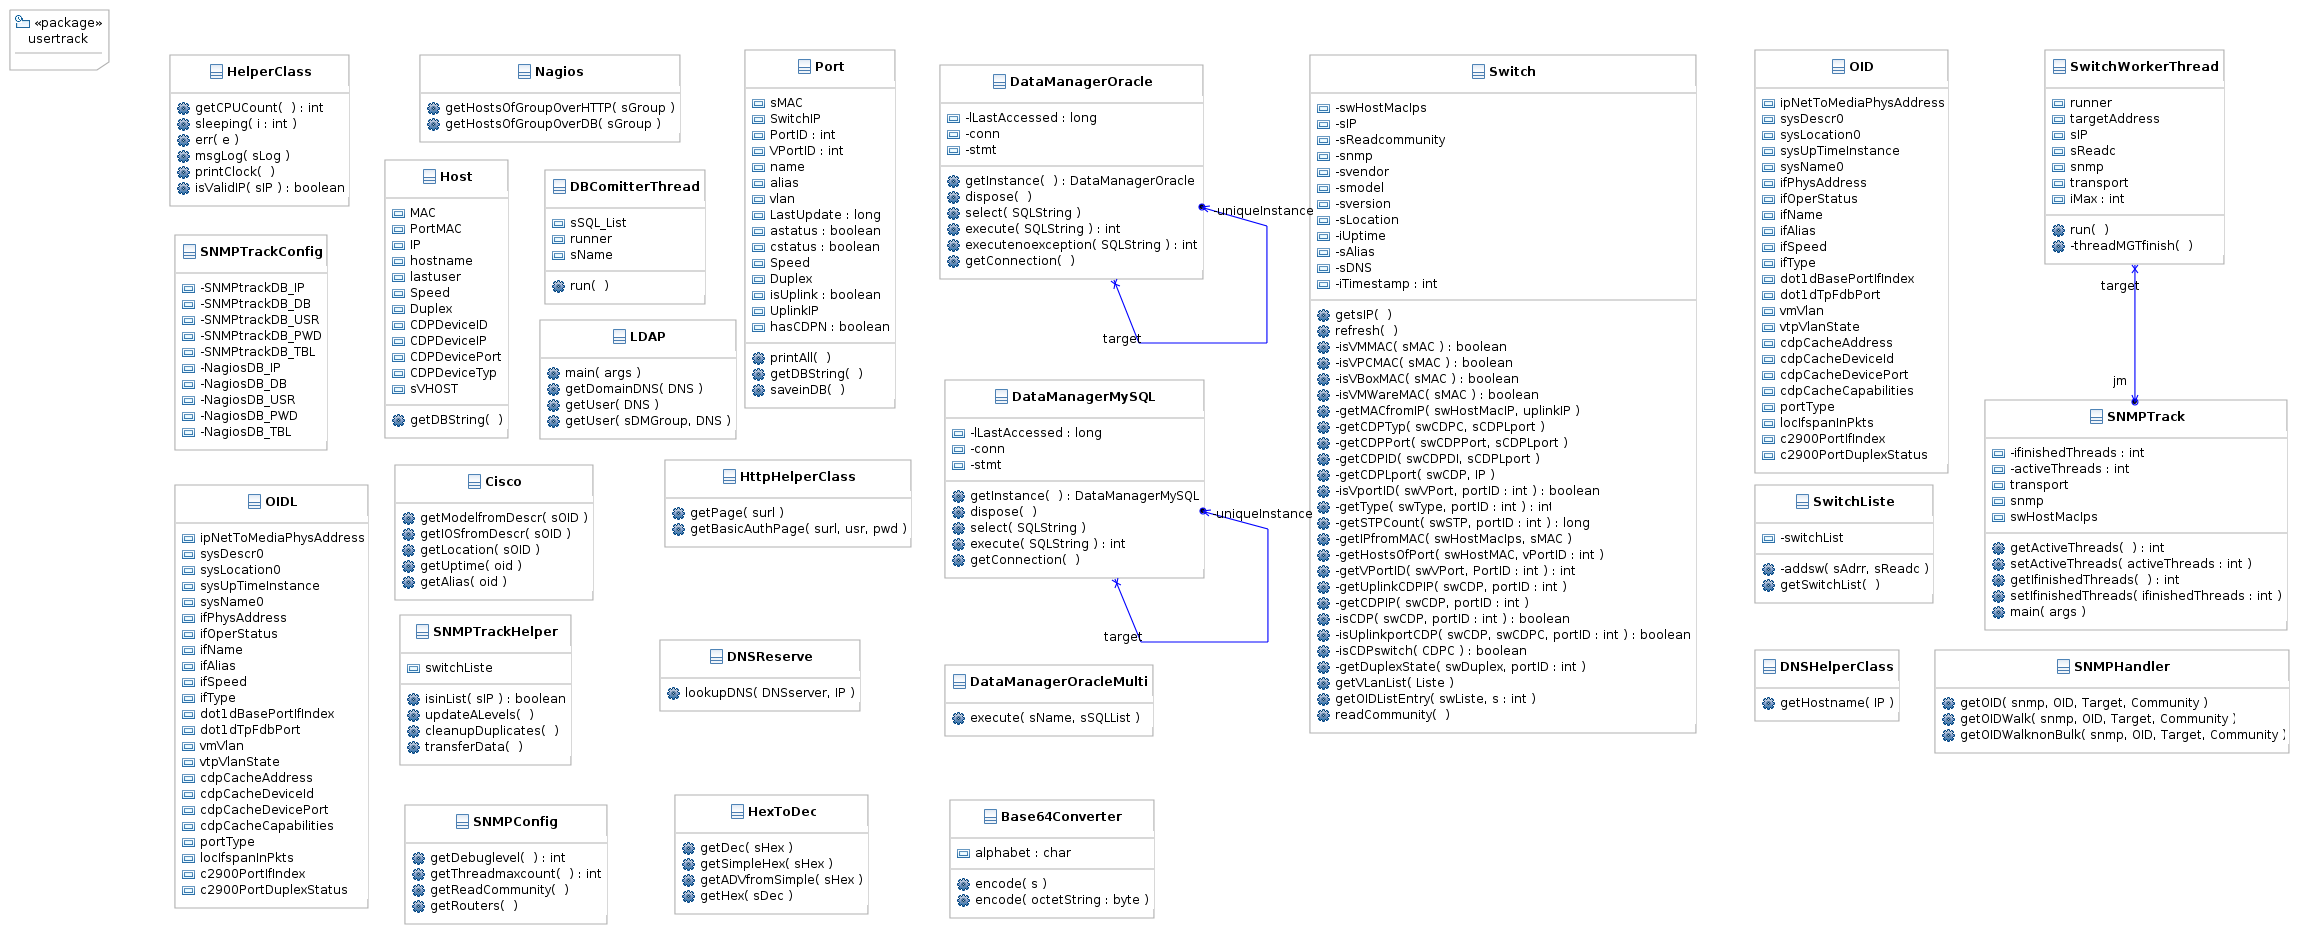
\includegraphics[width=0.8\textwidth]{model.png}
\caption{Klassendiagramm}
\label{fig:classdiagram}
\end{figure}

\subsection{Sequenzdiagramme}
\label{subsec:seqdiagrams}

Um die Beziehungen der einzelnen Klassen des Programms zu visualisieren reicht es nicht aus die Klassendiagramme zu zeichnen, sondern es müssen auch Sequenzdiagramme erstellt werden.
Im Folgenden soll auf die Beziehungen ausgehend von der Hauptklasse des Programms eingegangen werden.
Zu Beginn des Porgramms erzeugt die Klasse SNMPTrack ein Objekt der Klasse SwitchListe.
Bei diesem Objekt wird die Methode getSwitches() aufgerufen. Diese Funktion liefert dann eine Liste aller Switches, die später ausgelesen werden müssen anhand einer vorgegebenen Datenquelle aus. Zum aktuellen Zeitpunkt ist dies eine XML-Datei, in naher Zukunft werden diese Daten anhand des existierenden Nagios Systems ausgelesen. Im Anschluss wird ein Objekt der Klasse SwitchWorkerThread erstellt, um einen separaten Thread zu starten, der unabhängig und nebenläufig arbeiten kann. Dieser Thread nimmt das übergebene Switch Objekt und ruft bei diesem die refresh() Methode auf, welche wiederum für das Einlesen aller Switchinformationen zuständig ist. Dieser Vorgang ist in Abbildung X beschrieben.


\begin{figure}[H]
\centering
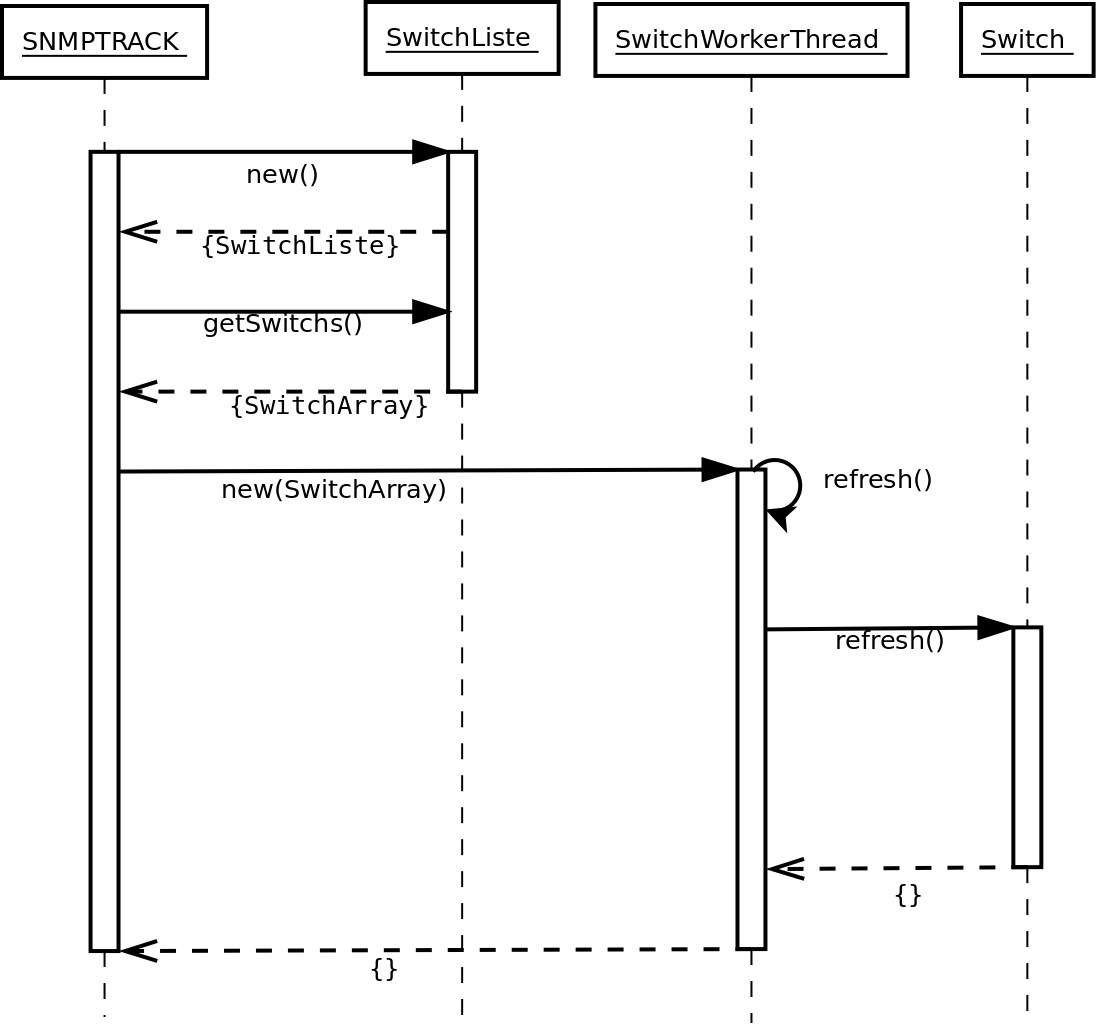
\includegraphics[width=0.5\textwidth]{seq.png}
\caption{Sequenzdiagramm1}
\label{fig:sequecediagram1}
\end{figure}

Während des refresh() Methoden-Aufrufs des Switch Objektes werden verschiedene andere Objekte erzeugt. Zu Beginn wird die Klasse SNMPHandler verwendet, welche verschiedene Methoden zur SNMP-Kommunikation zur Verfügung stellt. Über diese werden SNMP-GET und SNMP-BULK Befehle abgesetzt. Zusätzlich bietet die Klasse Funktionalitäten, welche SNMP selbst nicht zur Verfügung stellt. Möchte man z.B. den kompletten Unterbaum eines Konten erhalten und überschreitet die Anzahl der Einträge das Maximum von GETBULK, so können diese nur durch GET und GETNEXT ausgelesen werden. Diese Problematik behandelt die Klasse in einer SNMP-WALK Methode, welche die gleiche Funktionsweise wie ein GETBULK hat, aber es ermöglicht auch größere Listen an Werten abzufragen, die an einem Knoten hängen. Nachdem die jeweiligen SNMP Methoden die Werte zurückgegeben haben, werden diese ausgewertet. Im Anschluss daran, wird ein Objekt der Klasse Port abgeleitet. Dieses Objekt dient dazu die portspezifischen Informationen zu speichern und im Anschluss den passenden SQL-Befehl zur speicherung zu generieren. Dies wird durch die Methoden setValues() und saveinDB() realisiert.
Beim Aufruf der saveInDB() Methode kommt es zur Verwendung der Datenbank-Klasse JDBC-Oracle. Diese überträgt den SQL-String an die Datenbank, nachdem die Methode executeSQL() aufgerufen wurde.
Die gleiche Abfolge findet auch mit dem Objekt der Klasse Host statt. Hierbei werden anstatt wie beim Objekt der Klasse Port portspezfische Informationen abgelegt, sondern in diesem Fall die Informationen welche den jeweiligen Host betreffen abgespeichert.
Nachdem alle Ports und Hosts abgespeichert wurden ist die Methoden refresh() des Switch-Objektes beendet.\\
Jedoch muss bedacht werden, dass während der Verarbeitung der Daten eine Vielzahl von Klassen aufgerufen werden, welche speziell für das Programm geschrieben wurden. Ein Beispiel stellt die Klasse mit dem Namen Cisco dar. Welche Methoden zur Verfügung stellt, die speziell auf SNMP-Daten von Cisco-Geräten anwendbar sind. Darunter fallen Dinge wie Uptime-Formatierung. Model und IOS-Versions Auswertung anhand des 'System-Description'-SNMP-Strings.


\begin{figure}[H]
\centering
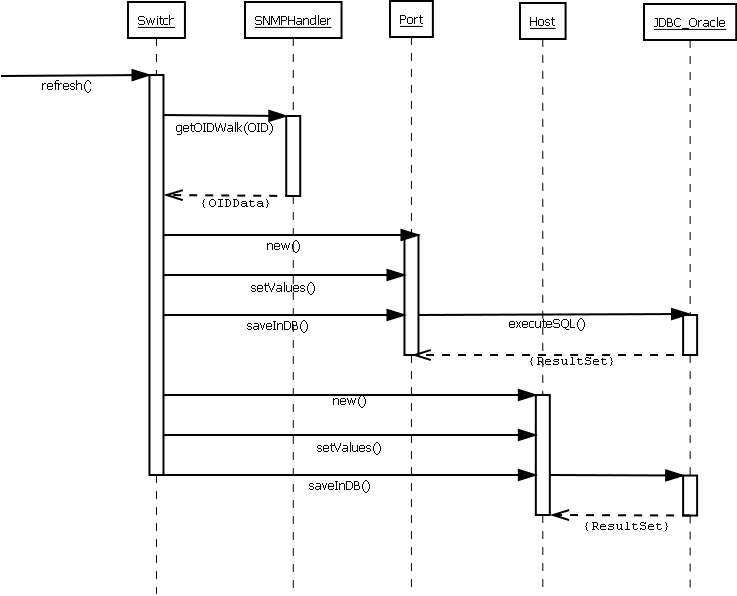
\includegraphics[width=0.7\textwidth]{seq2.png}
\caption{Sequenzdiagramm2}
\label{fig:sequecediagram2}
\end{figure}

\subsection{Aktivitätsdiagramme}
\label{subsec:acitvitydiagrams}

Zur Darstellung des Programmablaufs eigenen sich vor allem Aktivitäts-Diagramme von UML.
In Abbildung X ist ein solches Diagramm zu sehen.\\

\begin{figure}[H]
\centering
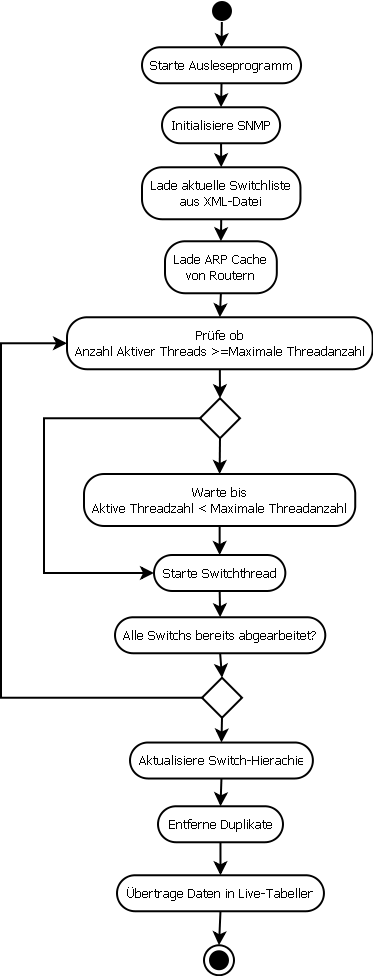
\includegraphics[width=0.5\textwidth]{activity_diagram.png}
\caption{Aktivitätsdiagramm1}
\label{fig:activitydiagram1}
\end{figure}

In dieser Abbildung ist der Ablauf des Hauptprogrammteils zu sehen. Dieser Programmteil soll im näheren angesprochen werden. Jedoch ist dabei zu beachten, das es sich bei der Darstellung um eine merkliche Vereinfachung des Programmablaufs handelt.\\
Zu Beginn des Programms wird die SNMP Schnitstelle initialisiert, da diese später allen Switch Threads übergeben werden muss. Im Anschluss wird die XML-Konfigurationsdatei der Switches ausgelesen. Dies ist notwendig zum einen um die definierte Liste der auszulesenden Switches zu erhalten, aber auch um zugehörige ReadCommunity auszulesen welche benötigt wird um Zugriff auf die jeweiligen Switches zu erhalten. Nachdem die Switch Liste eingelesen wurde per XML, wird nun per SNMP der ARP-Cache aller relevanten Router abgefragt. Dieser wird später benötigt in den Switch Threads, um eine Zuordnung zwischen MAC-Adresse und IP-Adresse herstellen zu können und anhand derer weitere Informationen wie DNS-Hostname zu erhalten.
Anschließend wird in einer Schleife geprüft, ob die Anzahl der aktiven Threads gleich oder höher der Maximalen Thread Anzahl ist. Ist dies der Fall wird eine Pause eingelegt bis die Anzahl der aktiven Threads gesunken ist und ein Thread gestartet. Dies dient dazu um sicherzustellen, dass nie mehr wie X Threads aktiv sind.
Dies ist vor allem in Hinblick auf die, während der Benchmarks festgestellten, Probleme wichtig. Während der Implementierungsphase wurde der Wert im Bereich 8-32 variiert und schließlich auf 10 gesetzt, welches als Sicherstellung dient, dass keine Verbindungsprobleme zum Oracle Server auftreten. Die Threads starten jeweils den Switch-Code, welcher im nächsten Paragraphen besprochen wird. Nach dem Durchlauf der Schleife wird gewartet bis alle Threads beendet wurden, da zuerst alle Hosts in der Datenbank abgelegt werden müssen um dann eine Duplikatserkennung durchführen zu können. Zuerst werden die Switch Hierachie-Levels anhand der Nagios-Datenbank aktualisiert, da diese ausschlaggebend für die Einordnung der Hosteinträge sind. Im Anschluss werden die Duplikate anhand eines Algorithmuses entfernt, welcher alle bekannten Duplikate untereinander vergleicht und bei bedarf “falsche” Hosteinträge löscht. Hierbei handelt es um Host die sich auf nicht identifzierten Uplinkports befinden. Die Problematik der Identifizierung des Uplinkports wurde bereits in Kapitel X angesprochen. Zum Abschluss werden die von den Duplikaten gesäuberten Daten in die sogenannten Livetabellen übertragen. Diese Übertragung ist notwendig, da es während des Auslesevorganges Inkonsistenzen im Hinblick auf die Verknüpfung der Beziehungen gibt und daher darf erst der “finale” Status in die Livetabellen übertragen werden. Durch diese Übertragung wird auch sichergestellt, dass während des Ausleseprozesses die Datenbank trotzdem nutzbar ist vom User und dieser keine Ausfallzeit des Systems bemmerkt.\\
Im Folgenden wird nun der Auslese Prozess etwas detaillierter für die Switch Threads beschrieben. Auch in diesem Fall gilt der Hinweis, dass es sich hierbei um eine starke Vereinfachung handelt, da das Abbilden der zusätzlich geschriebenen Algorithmen z.B. für das Erhalten der passenden Host-MAC-Adressen eines Ports den Umfang der Bachelor-Arbeit bei weitem übersteigt. 
Die Erste Überprüfung die durchgeführt wird, ist das Vorhanden sein von SNMP auf der entsprechenden IP. Ist dies nicht der Fall wird das Auslesen des vermeindlichen Switches mit einer Fehlermeldung abgebrochen und der Thread beendet. Im Anschluss dieser Überprüfung werden alle Informationen bezüglich des Switches ausgelesen. Das heißt Hersteller, Modell, IOS-Version, Uptime, Alias usw. . Im Anschluss wird der Switch spezifische SQL-Befehl generiert um die Informationen in die Datenbank abzuspeichern. Jedoch wird diese nicht direkt durchgeführt sondern in einem Stapel gesammelt. Der Grund hierfür liegt in der Reduzierung der Last des Datenbankservers, wie bereits in Kapitel X bei den Benchmarks entdeckt wurde, dass das Absetzten mehrerer Einträge auf einmal die Performence erhöht.
Im Anschluss werden alle Port relevanten Informationen abgefragt. 
Nachdem die Liste der VLANs ausgelesen wurden werden die VLAN spezifischen Listen zur MAC-Adressen Zuordnung geladen. Das heißt, für jedes auf dem Switch bekannten VLAN wird eine Abfrage an den Switch gestellt, welche Host-Adressen in dem jeweiligen VLAN mit den dazugehörigen Virtuellen Ports zurückliefert.
Nach dem alle SNMP-Daten nun ausgelesen und zwischengespeichert sind wird überprüft, ob der jeweilige Port eine MAC-Adresse hat und es sich hierbei auch nicht um eine virtuelle Schnittstelle handelt. Sofern dies der Fall sein sollte wird der Port ignoriert und der nächste bearbeitet. Im Normalfall wird der Bearbeitungs-Prozess anschließend fortgesetzt. Hierbei wird überprüft, ob der Port den Status Up oder Down hat und ob dieser, sofern der Status Up ist CDP-Informationen enthält.
Diese CDP Informationen werden bei Bedarf ausgelesen und es findet eine Überprüfung per Spanning-Tree-Protokoll statt, ob es sich hierbei um einen Uplink-Port handelt. Im Anschluss wird der jeweilige SQL-Befehl generiert und im Puffer abgelegt.
Nachdem die Informationen des Ports bekannt sind müssen die Hostinformationen ausgelesen werden. Hierzu wird als allererstes geprüft ob ein Endgerät an den Port angeschlossen ist. Ist dies nicht der Fall, wird das Auslesen der Hostinformationen abgebrochen und alle SQL Abfragen an die Datenbank übertragen. Sind jedoch Hosts vorhanden wird jeweils unterschieden, ob es sich hierbei um ein Uplink-Port handelt oder nicht. Im Falle des Uplink-Ports werden die CDP-Daten ausgewertet und diese als Host Eintrag hinzugefügt. Handelt es um keinen Uplinkport, so werden alle Hosts ausgewertet und für jeden Host die passende IP im ARP-Cache gesucht und aufgrund dieser IP der passende DNS-Hostname rekursiv abgefragt.
Im Anschluss wird, sofern es sich um ein Host mit Windows handelt, das Active Directory befragt, welcher Benutzer zuletzt am genannten Host angemeldet war. Auf Grundlage dieser Daten wird wiederum ein SQL-Befehl generiert, der anschließend dem Puffer hinzugefügt wird.
Bevor der Switch-Thread beendet wird, werden die Abfragen aus dem SQL-Puffer an einen speziellen Datenbank Thread übergeben der sich anschließend um das Absetzten der SQL-Befehle kümmert. So kann Der Switch Thread bereits beendet werden und das Auslesen des nächsten Switches beginnen, auch wenn noch nicht alle Datensätze in der Datenbank sind. Dies dient vor allem der Reduzierung der Wartezeit und somit einer Reduzierung der Auslesezeit.

\begin{figure}[H]
\centering
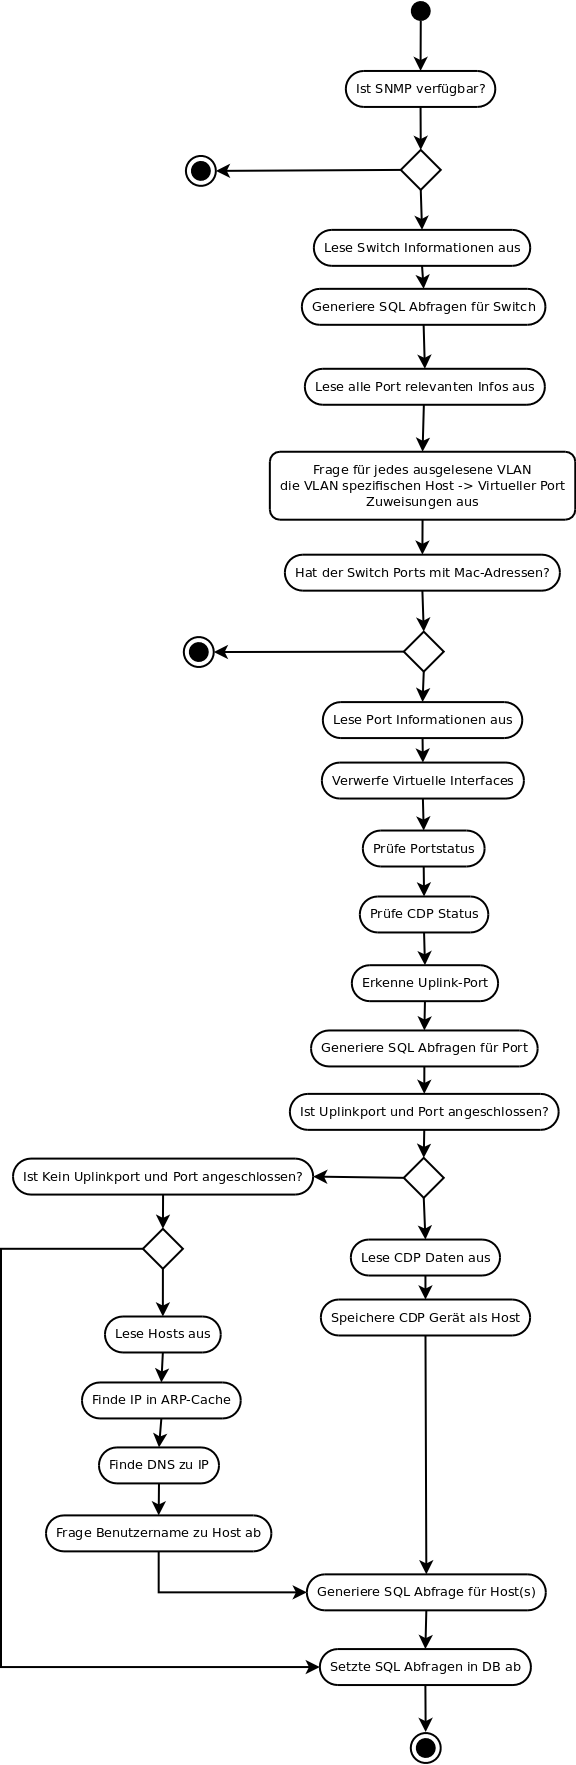
\includegraphics[width=0.5\textwidth]{activity_diagram_switch_thread.png}
\caption{Aktivitätsdiagramm2}
\label{fig:activitydiagram2}
\end{figure}

\subsection{ERM}
\label{subsec:erm-diagram}

Aufgrund der vorherigen Analysen ist ein Enitity Relationship Model erstellt
worden. Zum Erstellen wurde das Programm Dia verwendet, welches nicht der Chen
Notation folgt, aber eine einfache und schnelle Erstellung einer schemenhaften Abbildung ermöglicht und auch flexibel gegenüber Veränderungen ist.
Der Entwurf der Datenbank als ERM ist in Abbildung X zu sehen.

\begin{figure}[H]
\centering
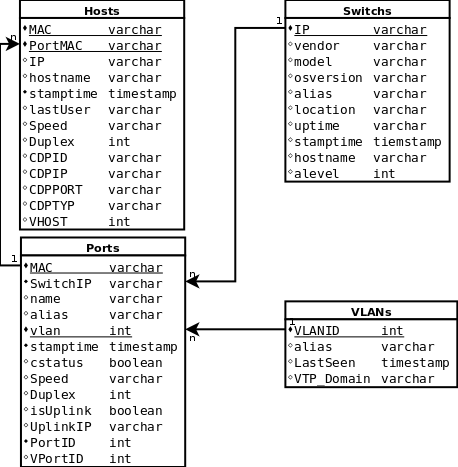
\includegraphics[width=0.5\textwidth]{ERM.png}
\caption{ERM}
\label{fig:erm}
\end{figure}

Um alle Daten verwalten zu können werden vier verschiedene Tabellen benötigt.\\
Zunächst wird eine Tabelle zum Speichern der VLAN-Informationen benötigt.
Hierzu existiert die Tabelle VLANs mit dem Primärschlüssel VLANID, welcher für jedes VLAN im Netwerk eindeutig ist und somit auch als Primärschlüssel geeignet ist. Über diesen Schlüssel werden alle VLAN relevanten Informationen abgelegt. Dazu gehören neben dem Namen bzw. Alias des VLANs auch die VTP-Domain und ein Zeitstempel, um unterscheiden zu können, welche VLANs eventuell in der Vergangenheit aktiv waren und in der Gegenwart nicht mehr existieren.\\
Die Tabelle Switches dient dazu, alle Switch relevanten Informationen zu speichern. 
Um den Switch eindeutig zu identifizieren reicht die IP Adresse des Switches aus. Über diese werden anschließend Informationen über den Switch gespeichert. Dazu gehören Dinge wie IOS-Version, Modell, Ort, Uptime, aber auch Hostname, sofern vorhanden und die entsprechende Hierachiestufe, welche anhand de Nagios-Systems ausgelesen wurde.\\
In der Port Tabelle werden alle Ports der Switches gespeichert. Die Ports selbst sind eindeutig über ihre jeweilige MAC-Adresse identifizierbar, jedoch soll ein neuer Eintrag angelegt werden, sofern sich die VLAN Einstellung ändert.
Daher dient nicht nur die MAC-Adresse als Primärschlüssel, sondern auch die VLAN ID.
Neben dem Namen des Ports und der MAC-Adresse gibt es auch ein Fremdschlüssel, welcher die IP des angehörigen Switches enthält um eine eindeutige Zuordnung des Ports an einen Switch zu ermöglichen.
Zusätzlich sind Attribute des Ports bezüglich des Status untergebracht.
So ist zum Beispiel möglich zu sehen, ob der Port gerade Up oder Down ist, mit welcher Geschwindgkeit auf dem Port kommuniziert wird und welcher Duplex Modus aktiv ist. Auch wird gespeichert, ob es sich bei dem Port um einen Uplinkport handelt.\\
In der Host Tabelle werden alle im Netzwerk befindlichen Hosts gespeichert.
Zur eindeutigen Identifikation der Hosts genügt die MAC-Adresse, jedoch geht aus der Anforderungsdefinition hervor, dass sofern der Host an einen anderen Port angeschlossen wird ein neuer Eintrag angelegt werden muss, daher wurde nicht nur die MAC-Adresse des Hosts, sondern auch die MAC-Adresse des Ports am Switch als Primärschlüssel genommen. Neben den üblichen Informationen wie IP und DNS-Hostname, werden auch Teile des Port Status abgespeichert, da man, sofern der Host an einem anderen Switch angeschlossen wird (z.B. ein Notebook der den Accesspoint wechselt), immernoch wissen möchte, mit welcher Geschwindigkeit dieser PC ursprünglich angeschlossen war. Es reicht aber auch schon das Suchen eines PCs der gerade ausgeschaltet ist. Um trotzdem herauszufinden mit welcher Geschwindigkeit dieser angeschlossen war ist diese Differenzierung notwendig. Zusätzlich dazu werden Informationen abgespeichert, sofern CDP Informationen über den Host bekannt sind. Hier werden dann CDP-Gerätetyp und der CDP-Port gespeichert, dies ist vor allem hilfreich bei Switches, Routern und Firewalls die das CDP Protokoll unterstützen um eine bessere Einordnung zu erhalten. Neben diesen Informationen wird im Feld VHOST zusätzlich vermerkt ob es sich bei diesem Host um einen physikalischen Host oder um ein logischen Host handelt. Das heißt, handelt es sich bei dem Host um einen virtuellen Server wird dieser explizit als Vhost markiert. Erkannt werden alle gängigen virtuellen Hosts. Dazu zählen mit VMWare, Virtualbox, VirtualPC, aber auch mit Parallels (Virtual Desktop, Server, Virtruzzo) oder Xen erzeugte Hosts. Zu beachten ist jedoch das z.B. das spezielle VMWare ESXi Server Betriebsystem selbst über eine virtuelle Schnittstelle kommuniziert, also das Host-System selbst und nicht die Gast-VMs.


\section{Design Entscheidungen}
\label{sec:designent}

Für die Umsetzung des Projektes müssen verschiedene Entscheidungen bezüglich der Umsetzung getroffen werden. Einige der Entscheidungen sind entweder durch die Anforderungen spezifiziert oder müssen unter Abwegung der Vor- und Nachteile ausgewählt werden.\\
Zuerst muss eine Entscheidung fallen, welche Programmiersprache gewählt wird. Nach dem Abgleich der Anforderungen und der Absprache mit der Fachabteilung, standen Perl und Java zur Auswahl. Da einer der Anforderungen auch die Geschwindigkeit betrifft, wurde zuerst eine Test Applikation in beiden Sprachen geschrieben. Dise hat jeweils einen Switch mit wenig Netzwerk-Traffic mit einer Vielzahl von SNMP Abfragen beschäftigt, um Benchmakrwerte zu erhalten.\\
Im Benchmark-Programm wird die Zeit gemessen, wie lange es dauert um 1000 Abfragen durchzuführen.
Der, in Millisekunden gemessene, Wert wird in die nachfolgende Formel eingesetzt:\\

Anzahl der Requests*1000/Benötigte Zeit in ms= Abfragen pro Sekunde\\

Daraus resultiert die jeweilige Anzahl der Abfragen pro Sekunde, welche es ermöglicht einen Vergleich durchzuführen.\\

In der nachfolgenden Grafik sind die beide Programmiersprachen aufgezeichnet:\\

\begin{figure}[H]
\centering
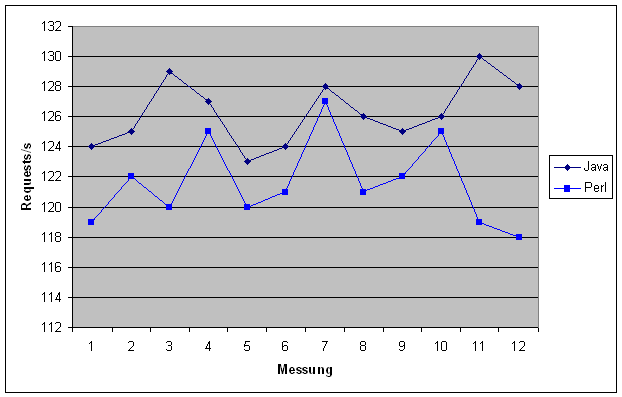
\includegraphics[width=0.8\textwidth]{bench_j_p.PNG}
\caption{Benchmark - Perl, Java}
\label{fig:benchperljava}
\end{figure}

Wie in der Grafik zu erkennen, liegt Java ein Bruchteil vor Perl. Der geringe Unterschied zwischen den beiden Programmiersprachen lässt sich dadurch erklären, dass die Implementierung der SNMP Abfragen minimal anders sind, der bei beiden fast gleich hohe Wert lässt darauf schließen, dass der Flaschenhals des Benchmarks der Switch selbst ist. Dies konnte dadurch validiert werden, wenn beide Benchmarks  gleichzeitig gestartet wurden und dann eine Halbierung beider Benchmark Werte erfolgte.\\
Da es somit kein Unterschied macht, welche der beiden Sprachen zum Einsatz kommt, wird die Entscheidung anhand der Möglichkeiten beider Sprachen und deren Modularität gefällt und somit fällt die Wahl auf Java.\\

Da unter Anderem eine Vielzahl an Switches abgefragt werden muss, empfiehlt es sich eine Parallelisierung anzustreben, da jeder Switch nur eine begrenzte Geschwindigkeit aufweist.
Hierfür eignet sich die Verwendung von Threads um den Teil der Abfragen zu parallelisieren der unabhängig voneinander ablaufen kann. Um den Nutzen einer Parallelisierung zu validieren wurde wiederum ein Benchmark durchgeführt. Bei diesem Benchmark wurde die Anzahl der Threads variiert und jeweils die Zeit gemessen.\\

\begin{figure}[H]
\centering
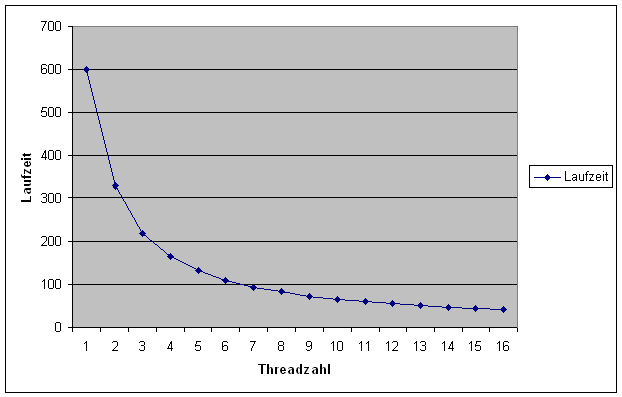
\includegraphics[width=0.8\textwidth]{bench_threads.PNG}
\caption{Benchmark - Parallelisierung}
\label{fig:benchparallel}
\end{figure}

Wie in der Grafik zu erkennen ist lässt sich feststellen, dass durch die Parallelisierung ein bedeutender Geschwindigkeitszuwachs zu messen ist.
Für die Abfragen pro Switch wurden jeweils 2000 Abfragen angenommen was ein geschätzer Maximalwert pro Switch später darstellen sollte.\\
Bei der Durchführung dieses Benchmarks wurde aber zugleich ein Problem erkannt und zwar kommt es zu Problemen bei Thread-Zahlen über 20. Hierbei reicht der UDP-Puffer für die SNMP Abfragen nicht mehr aus und somit kam der Empfang aller SNMP-Pakete nicht mehr sicher gestellt werden. Daher empfiehlt es sich bei der Implementierung ein niedrigeren Wert zu wählen und auf Nummer sicher zu gehen.\\
Bei der Version 2 des SNMP-Protokolls gibt es ein speziellen Abfrage Modus “BULKGET”. Bei diesem musste auch überprüft werden, in welchem Umfang dieser dem normalen GET ein Geschwindigkeitsvorteil bringt. Hierfür wurden der erste Benchmark angepasst und die Liste der Ports von einem Switch abgefragt, einmal alle Ports sequentiell und einmal per BULK.\\
Die Ergebnisse des Benchmarks lassen sich im nachfolgenden Bild erkennen.\\

\begin{figure}[H]
\centering
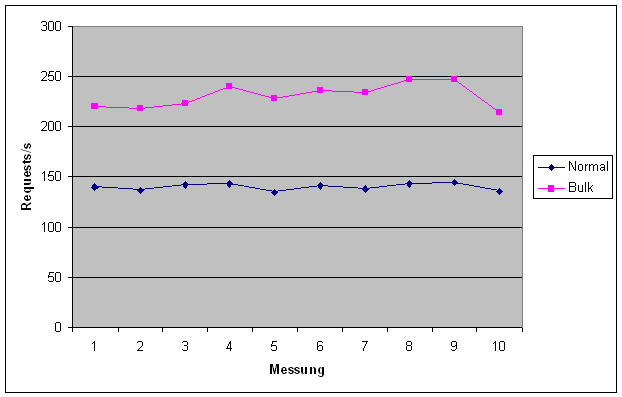
\includegraphics[width=0.8\textwidth]{bench_bulk.PNG}
\caption{Benchmark - SNMP Bulk}
\label{fig:benchsnmpbulk}
\end{figure}

Es lässt sich feststellen, dass der BULK Modus einen bis zu fünfachen Geschwindigkeitsvorteil bringt. Jedoch muss beachtet werden, dass im Falle einer größeren Anzahl von Antworten (ab 50) diese nicht vom BULK Modus zurückgegeben werden, daher ist der Einsatz nur partiell sinnvoll.\\
Hierbei muss bei der Implementierung dann genaustens beachtet werden, wann welche Methode eingesetzt werden kann.\\

Eine weitere Sache die überprüft werden muss ist die Abwegung, ob es sinnvoller ist die SQL-Befehle, welche neue Datensätze hinzufügen, zuerst zu sammeln und mit einem Commit abzusetzten oder jeden einzelnen Datensatz separat abzusetzen. Hierfür wurde ebenfalls ein Benchmark durchgeführt um eine Entscheidung in dieser Hinsicht treffen zu können.\\

\begin{figure}[H]
\centering
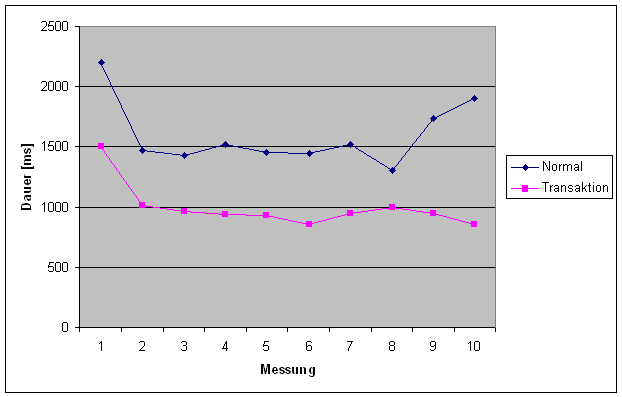
\includegraphics[width=0.8\textwidth]{bench_oracle.PNG}
\caption{Benchmark - Oracle Transaktionen}
\label{fig:benchoracletransactions}
\end{figure}

Wie in der Grafik zu erkennen ist es von Vorteil die Commits zuerst zu sammeln und dann abzusetzten.
Während des Benchmarks wurde jedoch erkannt, dass durch eine Vielzahl von vorgehaltenen Abfragen, die durch die Parallelisierung entstehen, die Anzahl der gleichzeitig offenen Tabellen Einträgen sich stark erhöht und somit das Limit der Datenbank überschreiten wird.
Zwar wurde anschließend das Limit der maximal offenen Einträge erhöht, jedoch kam es selbst dann zu Überschreitungen, daher wurde der Algroithmus so angepasst, dass er immer in Paketen zuje 100 Befehlen arbeitet. Durch diese Maßnahme ist es trotzdem möglich einen Geschwindigkeitsvorteil zu erhalten, bei gleichzeitiger Einhaltung der Limits.

\section{Auswahl der Hilfsmittel}
\label{sec:hilfsmittelwahl}

Für die Umsetzung des Projektes sind verschiedene Hilfmittel notwendig.\\
Zum einen wird eine Entwicklungsumgebung benötigt.
Da die Wahl der Programmiersprache auf Java gefallen ist und kommerzielle Lösungen nicht zur Auswahl stehen wurde sich für Eclipse entschieden, da es neben NetBeans zu den wenigen Open Source IDEs gehört, welche eine Vielzahl von Erweiterungsmöglichkeiten bietet und interaktive Funktionen wie Code-Vervollständigung oder Code-Vorlagen unterstützt aber auch standardmäßige Dinge wie Syntaxhervorhebung.\\

Zur Softwareversionverwaltung wurde Subversion verwendet. Dies ist eines in der Praxis am weitesten verbreiteten Systeme.\\
Die Auswahl wurde auf ein Open-Source System gelegt und zusätzlich auf ein zentrales System um ein großes Maß an Interpolität zu erreichen. Die Wahl fiehl speziell auf Subversion, da es im Gegenzug zu CVS das Versionsschema nicht auf einzelene Dateien sondern auf das ganze Projekt bezieht. Das hat den Vorteil, dass das Hinzufügen einer neuen Funktion nicht in der Hauptklasse Version 50 und in der Methodenklasse Version 70 gespeichert wird. Somit wäre kein Zusammenhang erkennbar. Bei Subversion hingegen kann dies direkt erkannt werden, da die neue Funktion in der Revision 33 in beiden Dateien erkennbar ist.\\

\section{Schnittstellen}
\label{sec:schnitt}

Um ein Projekt mit vielen Einlese und Export Funktionalitäten erstellen zu können, werden viele Schnittstellen benötigt.
Zum einen wird bei diesem Projekt eine Schnittstelle für die SNMP Abfragen benötigt, zum anderen wird eine Anbindung an das Active Directory angestrebt. Zusätzlich müssen aber auch alle Datenbankzugriffe sowohl vom Einleseprogramm, als auch von der Website bewerkstelligt werden.\\
Im Folgenden wird auf die jeweiligen Schnittstellen eingegangen, wie diese sequentiell im Ablauf des Ausleseprogramms verwendet werden. Diese lassen sich wiefolgt zusammenfassen:\\
\\
Einlesen aller benötigten Konfigurationsdaten\\
Auslesen per SNMP\\
Rekursive DNS Abfragen\\
Auslesen per LDAP\\
Datenbankverbindung Java\\
Datenbankverbindung Webserver\\


Die erste Schnittstelle ist beim Start des Programmes zum Auslesen der Daten angesiedelt. Hierbei muss der Benutzer dem Programm eine Großzahl von Informationen übergeben.\\
Es existiert eine spezielle XML-Datei in der die Switches, welche ausgelesen werden müssen, die Router, welche den ARP-Cache enthalten, sowie die notwendigen Zugangsdaten für die Datenbanken, enthalten sind. \\
Das Programm selbst bietet dem Nutzer keine Möglichkeit Übergabe-Parameter zu definieren, damit ein möglichst einfacher Ablauf ermöglicht und zusätzliche Fehleingaben des Benutzers vermieden werden.\\
Die nächste Schnittstelle ist die Kommunikation mit den Switches per SNMP. Um nicht die komplette SNMP-Kommnuikation selbst per UDP implmentieren zu müssen, emfiehlt es sich hierbei eine bereits vorhandene API zu nutzen.\\
Speziell für Java gibt es hierfür mehrere Möglichkeiten (keine vollständige Liste):\\
SNMP4J\\
jSNMP\\
WebNMS SNMP\\
iReasoning SNMP API\\
netsnmpj\\


Schließt man nun alle kommerziellen Lösungen aus, so bleiben lediglich SNMP4J und netsnmpj übrig.
Da mehrere SNMP Abfragen später gleichzeitig durchgeführt werden müssen ist die Wahl auf SNMP4J gefallen, da dieses threadsicher ist und auch ein größeren Funktionsumfang wie netsnmpk bei der Implementierung mitsichbringt.\\
Um anhand der ermittelten IP-Adressen die dementsprechende DNS-Namen zu erhalten ist es notwendig ein Reserve DNS-Lookup zu machen. Hierfür muss das sogennante JNDI verwendet werden, welches einem erlaubt selbstdefinierte DNS-Abfragen zu erstellen.\\
Um beispielsweise den DNS-Namen der IP 192.168.0.1 herausfinden zu können muss dieser aber erst in ein spezielles Format gebracht werden. Hierzu wird die IP Adresse umgekehrt zu 1.0.168.192 und der Zusatz “.in-addr.arpa” angehängt. Daraus folgt dann:\\

1.0.168.192.in-addr.arpa\\

Diese Adresse wird inklusive dem Modus “PTR”, welche für einen Reserve-DNS-Lookup steht, an den DNS Service Provider übermittelt und das Resultat wiederum zurückgegeben.\\

Für das Auslesen des zugehörigen Benutzers muss das Active Directory befragt werden, hierzu gibt es eine Mehrzahl von Möglichkeiten, die jedoch dadurch eingeschränkt werden, dass diese nur unter Windows lauffähig sind. Daher muss auf Ansätze zurückgegriffen werden bei denen es möglich ist Plattformunabhängig zu agieren. Hierzu muss man die Architektur vom Active Directory von Windows genauer untersuchen.\\
Generell lässt sich das Active Directory in folgende Komponenten unterteilen:\\
\\
LDAP-Verzeichnis\\
Kerberos-Protokoll\\
Common Internet File System\\
Domain Name System (DNS)\\


Hiervon ist vor allem das LDAP-Verzeichnis interessant, welches es ermöglicht den Benutzer des jeweiligen Computers herauszufinden.
Da LDAP per RFC genaustens spezifiziert ist (aktuell im RFC 4511) und Microsoft diesen Standard ebenfalls nutzt kann mit einer LDAP-API auf das Verzeichnis zugegriffen werden.\\
Hierfür bietet Java mit seinen enthaltenen Bibliotheken ebenfalls eine Schnittstelle ähnlich der DNS-Abfragen an. Über diese können die Attribute eines Objektes im Verzeichnis abgefragt und gesetzt werden. In diesem Verzeichnis befinden sich auch die einzelnen Computer als Objekte. Diese wiederum haben diverse Attribute, welche unter Anderem auch den aktiven Nutzer enthalten.\\
Für die Verbindung des Java-Programms zur Oracle und MySQL-Datenbank gibt es verschiedene Möglichkeiten. Hierzu zählen die verschiedenen Arten von Treibern, die eine Datenbankverbindung ermöglichen. Zu allererst ist die ODBC-Schnittstelle zu nennen welches es ermöglicht unabhängig von der eingesetzten Datenbank, die Anbindung an das Programm immer auf die gleiche Art zu realisieren zu können. Da diese Unabhängigkeit dadurch erreicht wird, dass Befehle erst in die Datenbankspezifischen umgewandelt werden müssen und somit ein Overhead entsteht, ist diese Lösung meist langsamer wie eine native Lösung. Daher ist es von Vorteil spezielle vom Hersteller angebotene JDBC-Treiber einzusetzten, welche anstelle des JDBC-ODBC Brücken-Treibers den zusätzlichen Overhead meiden und direkt mit dem DBMS kommunizieren.\\
Bei der Verbindung mit dem Webserver kann wiederum ein ODBC-Treiber einsetzt werden oder speziell für die Programmiersprache PHP geschriebene Bibliotheken, die es erlauben, ähnlich wie bei Java direkt mit dem DBMS zu kommunizieren um unnötigen Overhead zu vermeiden.\\

\section{Zeitplan}
\label{sec:timetable}

Für die Umsetzung eines Softwareprojektes ist nicht nur ein Entwurf notwendig, sondern auch die Planung über den zeitlichen Ablauf. Der Faktor Zeit spielt eine wichtige Rolle, da er die beiden Variablen Qualität und Kosten begrenzt. Da bei diesem Projekt keine externen Kosten anfallen werden, kann dieser Punkt des magischen Dreiecks außenvor gelassen werden.
Aufgrund der sehr knappen Zeit war es vor allem wichtig einen zuvor definierten Plan zu haben, welcher die genauen Schritte spezifiziert. Um einen Überblick über den Umfang des Projektes zu bekommen, lohnt sich wiederum ein Blick auf die Usecases in Kapitel X, sowie die Anforderungsdefinition in Kapitel Y. Diese bilden eine gute und wichtige Basis um einen Projektstrukturplan zu erstellen, welcher im Projektmanagement eine wichtige Rolle spielt. Aufgrund dieses Planes ist es möglich die einzelnen Arbeitspakete zu definieren. Eine Zuordnung der Arbeitspakete zu einer Person muss nicht erfolgen, da die Software nur von einer Person entwickelt und umgesetzt wird. Nachdem die Arbeitspakete definiert wurden, mussten diesen jeweils eine Dauer zugewiesen und die jeweiligen Abhängigkeiten angegeben werden.
Bei den Zeitangaben wurden Näherungswerte von bereits umgesetzten Projekten verwendet, jedoch muss bedacht werden, dass neben dem kompletten Verlauf der Entwicklung gleichzeitig immernoch ein Lernprozess, sowie das Dokumentieren und das Schreiben der Bachelor-Arbeit stattfindet.  Normalerweise kann eine Ressource (in diesem Fall ein Mitarbeiter) nur immer einem Arbeitspaket aktiv zugewiesen werden, alle anderen Arbeitspakete können immer nur einzeln und nacheinander abgearbeitet werden, nie aber parallel. Aus diesem Grund wurde auch auf eine ausgiebige Planung der Resourcen verzichtet. Viel wichtiger war hingegen die Terminplanung, welche aufgrund der Angaben (Dauer und Abhängigkeiten) anhand der Arbeitspakete erstellt werden kann.\\
Im nachfolgenden sieht man in Abbildung X den Terminplan für das Projekt.\\

\begin{figure}[H]
\centering
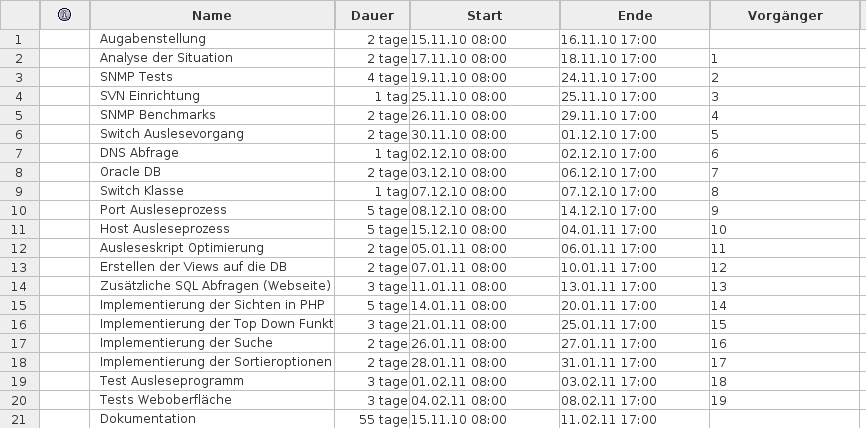
\includegraphics[width=0.9\textwidth]{netzplan1.png}
\caption{Zeitplan - Arbeitspakete}
\label{fig:benchsnmpbulk}
\end{figure}

Anhand des Terminplans kann wiederum ein Gantt-Diagramm erzeugt werden, welches einen grafischen Überblick über alle Arbeitspakete, sowie deren zeitliche Einordnung, ermöglicht. Das passende Gantt-Diagramm zum Projekt ist in Abbildung X zu sehen

\begin{figure}[H]
\centering
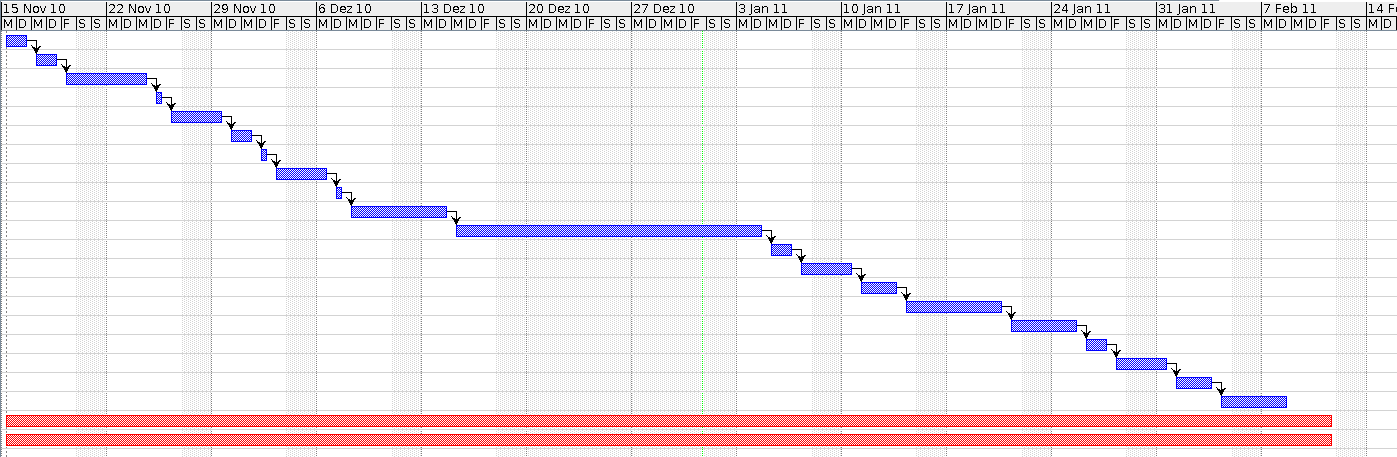
\includegraphics[width=0.9\textwidth]{netzplan2.png}
\caption{Zeitplan - Ganttdiagramm}
\label{fig:benchsnmpbulk}
\end{figure}

In diesem ist sehr leicht erkennbar, dass das Projekt einen konstanten sequentiellen Ablauf hat.
Zwar hätte die Möglichkeit bestanden ein paar einzelne Arbeitspakete parallel aufzuführen, jedoch in Verbindung mit dem bereits angesprochenen Problem, dass nur eine Person an der Umsetzung arbeitet und diese ein Arbeitspaket nach dem anderen abarbeitet, keine zeitliche Möglichkeit für eine Parallelisierung gegeben ist.
Zu beachten sind auch die zwei rot gefärbten Balken am unteren Ende des Diagramms, welche als kritischer Pfad angedeutet sind. Hierbei handelt es sich um die Dokumentation und das Schreiben der Bachelor-Arbeit. Diese werden zwar als kritische Pfade angezeigt aber da die Umsetzung des Projektes sequentiell voranschreitet, ist diesem keine weitere Betrachtung zu schenken. Die Bachelor-Arbeit hat ein fest definierten End-Zeitpunkt und ist als solcher nicht verschiebbar. Die Zeiten der einzelnen Arbeitspakete hingegen sind flexibeler anzusehen, jedoch gibt es hierbei auch die Einschränkung, dass diese in Summe nicht den Endtermin überschreiten dürfen.

\section{Realisierung}
\label{sec:implementation}

Nachdem sowohl die Umsetzung als auch der zeitliche Ablauf im Detail geplant wurden, konnte mit der Implementierung und somit mit der Realisierung des Projektes begonnen werden.
Zu erst wurde ,wie im Zeitplan definiert, das Ausleseprogramm umgesetzt und im Anschluss die dazugehörige Webseite.\\
Realisiert wurde das System auf einem Virtuellen VMWare Server mit dem Betriebsystem OpenSuse (Linux). Als Webserver diente Apache 2 in Verbindung mit PHP 5.3.2. Die PHP Version wurde speziell mit einer Oracle Datenbank Anbindung kompiliert.
Auf diesem Server lief zusätzlich neben dem Webserver ein Oracle Datenbankserver in der Enterprise Edition in Version 11g R2.\\
Das Ausleseprogramm selbst läuft Betriebsystem unabhängig und mit einer beliebigen Java Version ab dem Jahre 2006. Zusätzlich ist es unerheblich ob das Programm mit der original Sun Java VM ausgeführt wird oder mit dem quelloffenen OpenJDK, welches bevorzugt in Linux-Distributionen eingesetzt wird.
Beim Start des Ausleseprogramms wird zunächst überprüft, ob die Datei Switch.xml existiert und bei Bedarf diese ausgelesen, welche wiederum die Switches inklusive deren Read-Community enthält. Ist die Datei nicht existent, werden die auszulesenden Switches anhand der Nagiosdatenbank ausgelesen. Die Daten für die Nagiosdatenbank, sowie für die Oracle Datenbank in der später die Informationen abgelegt werden befinden sich in der config.xml. Diese enthält neben der maximalen Threadanzahl auch die Einstellung für den SNMP Intervall, der in Kapitel X angesprochen wurde. Dieser Intervall dient zur Reduzierung der Last auf den Switches während des Auslesevorgangs. In dieser Konfigurationsdatei ist ebenfalls ein Parameter zu finden, welcher es ermöglicht ein Debuglevel zu setzten. Je nach Höhe dieses Levels werden nicht nur Fehler sondern auch Warnungen, Hinweise oder auch Meldungen ausgegeben. Die Levels lassen sich wiefolgt einordnen:\\
\\
Level 0: Anzeige von Fehlern\\
Level 1: Zusätzliche Anzeige von Warnungen\\
Level 2: Zusätzliche Anzeige von Hinweisen\\
Level 3: Alle Meldungen\\
\\
Zusätzlich werden alle Meldungen die per Programm ausgegeben werden auch in der Log-Datei gespeichert. Diese Meldungen sind abhängig vom Loglevel.
\\
\begin{figure}[H]
\centering
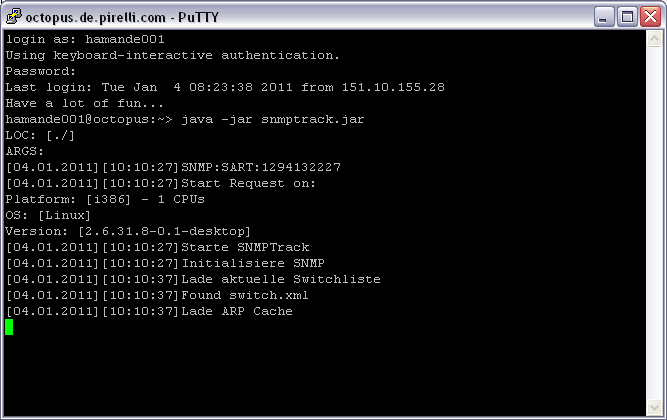
\includegraphics[width=0.8\textwidth]{snmptrack_start.png}
\caption{Programm - Auschnitt}
\label{fig:show_s1_s2_p1_n1}
\end{figure}
In Abbildung X ist der Start des Programms zu sehen. In diesem ist auch zu erkennen, dass keinerlei Parameter übergeben wurden. Dies wurde in der Art realisiert um Bedienfehler zu vermeiden und die Ausführung per Skripte zu erleichtern. Zusätzlich werden Fehlerhafte Einträge innerhalb der XML-Dateien einfach ignoriert.\\
Die Weboberfläche des Systems wurde per PHP realisiert. Zusätzlich kommen Cascading Style Sheets und Java Script zum Einsatz. Um die Zeit für die Implementierung zu veringern, wurde auf die freie CMS Tints zurückgegriffen \footnote{http://sourceforge.net/projects/tints-system/}.
\\
\begin{figure}[H]
\centering
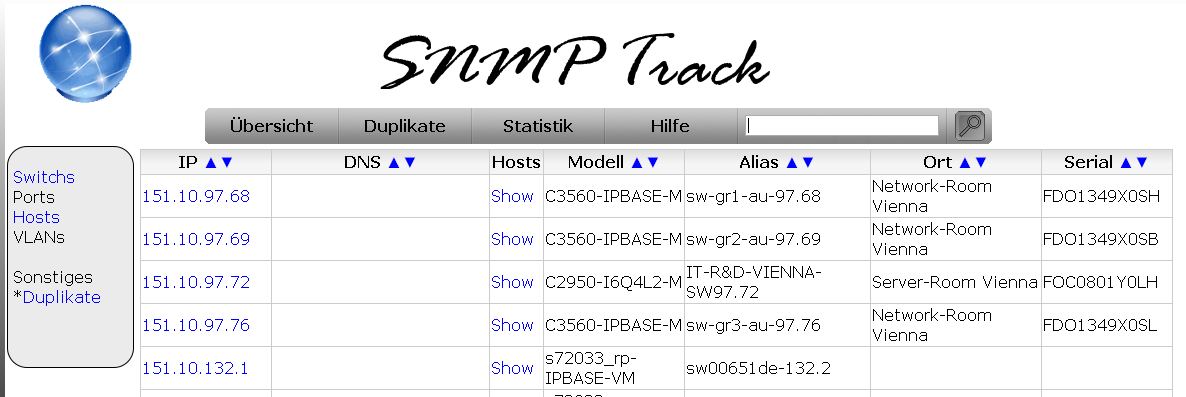
\includegraphics[width=1.0\textwidth]{snmptrack_overview.png}
\caption{Programm - Auschnitt}
\label{fig:show_s1_s2_p1_n1}
\end{figure}
Die Oberfläche während der Entwicklung ist in Abbildung X zu sehen.
Neben dem Grundgerüst für die Darstellung der Tabellen müssen spezielle SQL-Abfragen erstellt werden, da später eine Sortierung aller Spalten möglich sein muss.
Diese Sortierung wird durch die Übergabe der GET-Parameter realisiert. Klickt der Benutzer auf eine Spalte wie in Abbildung X zu sehen, so wird der GET-Parameter ‘sort’ in folgendem Format übergeben:\\
\\
sort=model\_A\\
\\
Hierbei stellt ‘model’ 1:1 den Spaltennamen der zu sortierenden Spalte dar und 'A' gibt die Sortierrichtung an. In diesemfall steht A für das englische Wort ‘ascending’, d.h. aufsteigend. Für eine Absteigende Sortierung wird ‘D’ angegeben für ‘descending’.
Zusätzlich gibt es in der Weboberfläche die Möglichkeit sich Duplikate in der Datenbank anzeigen zu lassen. Hierbei handelt es sich um Rechner die auf 2 unterschiedlichen Ports im Netzwerk auf der selben Switch-Ebene gefunden wurden. Bei diesen Einträgen handelt es sich um 90\% der Fälle um Hosts die sich im Netzwerk bewegen. Ein Großteil dieser sind entweder Notebooks die per WLAN die Access Points wechseln oder ein Computer, der die Abteilung wechselt.

\section{Probleme bei der Implementierung}
\label{sec:probimp}

Während der Implementierung traten verschiedene Probleme auf, welche berücksichtigt werden mussten in der Implementierung, um abschließend trotzdem die gewünschten Anforderungen alle Umsetzen zu können.
Die Probleme lassen sich vor allem zu den Folgenden Punkten Einordnen:\\
Zuordnung Host --> Switchport\\
Verwendete VLANs (“unsichtbare VLANs”)\\
Uplinkport-Identifizierung\\
Differenzierung der Switchlevels\\
SNMP Abfragen und CPU-last auf den Switches\\


Als erstes Problem ist die genaue Zuordnung zwischen Host und Switchport zu nennen.
Hierbei hat sich während der Implementierungsphase gezeigt, dass die Daten, welche per SNMP auslesbar sind, nicht denen gleichen, die lokal auf den Switches per Telnet über das Cisco System zu erhalten sind. So kann das Cisco System einem direkt anzeigen welche Mac-Adressen sich hinter welchem Port verbiergt. Über SNMP sind diese Informationen jedoch nicht direkt erhaltbar, hier müssen erst verschiedene abrufbare “Tabellen” verknüpft werden. Als erstes müssen die verwendeten VLANs des Switches abgefragt werden (die Problematik der VLAN Abfrage wird im anschließenden Paragraphen erläutert). Danach muss eine Liste der Mac-Adressen auf den virtuellen Ports pro VLAN abgefragt werden. Diese einzelnen Listen müssen miteinander kombiniert werden und alle Duplikate entfernt werden. Im Anschluss muss diese Liste mit einer weiteren Liste, welche die Zuordnung zwischen Port und virtuellen Port enthält verknüpft werden. Aufgrund dieser Liste kann dann eine Verbindung zwischen Mac-Adresse des Ports und der Mac-Adresse des Hosts hergestellt werden. Durch diese Komplexität steigt die Anzahl der Abfragen deutlich um die gleichen Informationen zu erhalten.\\
Eine weitere Problematik stellte sich beim Auslesen der verwendeten VLANs. Es gibt die Möglichkeit per SNMP eine Liste abzufragen, welche einem ermöglicht das verwendete VLAN für den jeweiligen Port zu erhalten. Ports die mehrere VLAN Zuordnungen haben werden nicht angezeigt und sind Trunk-Ports, welche eigentlich Uplink-Ports sind bzw. an solche angeschlossen sind. In diesem Zusammenhang stellt sich die Problematik, dass es passieren kann, dass zwar ein Port für eine spezielles VLAN fesgelegt wurde, jedoch sich dahinter noch ein VOIP-Telefon befindet, dass über ein “nicht sichtbares” VLAN kommuniziert, welches über die Liste im SNMP nicht erkennbar ist. Um trotzdem an die Mac-Adresse des VOIP-Telefons zu bekommen, müssen alle im Netzwerk bekannten VLANs an einem Switch abgefragt werden, was wiederum die Anzahl der Abfragen erhöht, aber auch eine Problematik mit sich bringt. In diesem Zusammenhang gibt es spezielle Cisco spezifische VLANs die sich im Bereich 1002-1005 befinden, welche ausgeschlossen werden müssen, da eine Abfrage der MAC-Adressen dieser VLANs zu einem Timeout führt und unnötig den Ausleseprozess verzögert.\\
Eine weitere Problematik stellt sich in der Identifizierung der Uplink-Ports an den Switchen. Hier gibt es keine einfache anwendbare Regel. Zuerst wurde angenommen, dass jeder Trunk Port ein Uplink Port ist. Diese Annahme war jedoch falsch, da in dem Vorher aufgeführten Beispiel sich dahinter auch ein durchgeschleifter Computer an einem VOIP-Telefon befinden kann. Daher scheidet das Attribut “Trunk-Port” als solches zur Identifizierung aus. Das nächste Attribut, welches ausgewählt wurde, ist ein spezielles Cisco spezifisches Protokoll mit dem Namen CDP. Es dient dazu Cisco Geräte an einem Port zu Identifizieren. Um einen Uplink Port zu identifizieren wurde dann angenommen, dass sofern das Protokoll CDP vorhanden ist, es sich hierbei um einen Switch handelt. Hier stellt sich jedoch die Problematik, dass es auch Geräte gibt die auf CDP antowrten, welche weder Switches noch Router sind. Ein Beispiel sind VOIP-Telefone, die es auch von Cisco gibt. Daher wurde zusätzlich die Typerkennung des CDP Gerätes abgefragt, welche Auskunft über diverse Eigenschaften des Gerätes gibt. Über diese kann überprüft werden, ob es sich hierbei um einen Switch handelt. Leider hat sich in der Praxis gezeigt das dieses nicht vollständig ausreicht, da nicht alle Switches sämtliche Abfragen unterstützen, somit musste nach einer zusätzlichen Identifikationsmöglichkeit gesucht werden. Hier wurde auf das Spannign Tree Protokoll gestoßen, welches zur Kommnuikation zwischen den einzelnen Switches dient, um unter Anderem Pfadkosten der einzelnen Verbindungen auszutauschen. Nun wurde per SNMP die Anzahl der ausgehenden STP-Pakete auf dem jeweiligen Port ausgelesen und dieses als weiteres Kriterium eingeführt, über welches eine Identifikation des Portes ermöglicht wird und zusammen in Kombination mit CDP eine sehr verlässliche Identifikation zur Verfügung stellt.\\
Ein weiteres Problem hat die Einordnung der Hierachie Ebenen der Router dargestellt. Um Duplikate reduzieren zu können, ist es notwendig zu wissen, ob die MAC-Adresse eines Hosts auf einem Uplink/Downlink Port eines Switches erkannt wurde oder an seinem normalen Port. Hierzu muss man wissen, ob der Switch ein Access-Switch ist oder ein Switch einer höheren Ebene.\\

Die Hosts im Netzwerk sind, mit einer geringen Anzahl von Ausnahmen, alle an Access-Switche angeschlossen. Zusätzlich gibt es Endgräte die auch an die Distribution-Switches angeschlossen sein können, z.B. die Server im Rechenzentrum. 

Um diese Problematik lösen zu können wurde überlegt, die Hierachie Ebenen jeweils numerischen äquivlanten Zahlen zuzuordnen. Hierzu wurden die Core Switches mit der Zahl 0, die Distribution Switches mit der Zahl 1 und die Access Switches mit der Zahl 2 definiert.\\
Da die Information der Ebene des Switches nicht direkt von diesen selbst auslesbar ist, gibt es effektiv nur zwei Möglichkeiten. zum Einen kann man die komplette Hierachie anhand der Uplink Ports mit einem Programm logisch ab bilden und manuell einen Hauptknoten auswählen anhanddessen dann eine Einordnung der Switches erfolgt, was jedoch äußerst komplet ist und den Zeitlichen Rahmen de Projektes sprengt, daher wurde auf die zweite Möglichkeit zurückgegriffen, nämlich diese Informationen extern von einer anderen Quelle einzulesen.\\
Hierzu wird das bereits existierende Nagios System im Unternehmen verwendet. Zu diesem wird mittels JDBC zu einer MySQL Datenbank eine Verbindung aufgebaut, über diese dann im Anschluss die Gruppen Informationen der zu kontrollierenden Hosts, in diesem Fall der Switches, ausgelesen werden. Die Switches sind in verschiedene Host-Gruppen einsortiert, unter Anderem auch in die benötigten Access, Distribution und Core Hierachien. Über diese Gruppen werden die jeweiligen Hosts bzw. Switches erfasst und deren Hierachielevel in der Datenbank eingetragen.\\
Neben den hauptsächlich logischen Probleme zur Identifikation stellte sich unter Anderem noch ein weiteres Problem heraus bei der Abfrage der Informationen per SNMP.\\
Wie bereits in vorherigen Kapitel angedeutet, werden die auszulesenden Switches besonders belastet bei SNMP Abfragen, weshalb eine Erhöhung der Anzahl der Abfragen stehts kritisch bewertet wurde in den Ausführungen. In den Beschreibung zur Zuordnung zwischen MAC-Adresse des Hosts und der Mac-Adresse des Swicths von Cisco, wird diese Problematik nicht angesprochen, jedoch gibt es von Cisco weitere Informationen zu der Problematik, speziell bei einem Artikel zum Auslesen der CPU-Last per SNMP. In diesem wird angeführt, dass die Abfrage des Wertes selbst zu einer Verfälschung des Wertes führt. Zudem wird empfohlen nicht mehr als 1 Abfrage pro Sekunde per SNMP auf einen Switch zu machen, da geringere Intervalle bereits zu Beeinträchtigungen führen. Vergleicht man dies mit den Benchmarks aus Kapitel X, so lässt sich feststellen, dass diese Grenze um ein hundertfaches überschritten wird beim Ausleseprozess. Es muss auch bedacht werden, dass die Switches nicht für solche Operationen konzipiert wurden, sondern vielmehr für ihre eigentliche Aufgabe, insofern ist das Ziel die Last auf den Switches möglichst gering zu halten, um den Netzwerk-Betrieb in keinster Weise zu beeinflussen. Aufgrund eines logischen Fehlers im Programmablauf kam es während diverser Tests dazu, dass einer der Core-Switches übermäßig ausgelastet war und dies dazu geführt hat, dass das Überwachungsystem der Switches anschließend Warnungen versendet hat. Solche Fälle dürfen im Betrieb nicht passieren, da die Ursache für die hohe Last der Switches nicht erkennbar ist und neben der Störung des Betriebes auch zusätzlich für Verwirrung sorgt. Daher ist es wichtig, die Anzahl der Abfragen per SNMP auf ein Minimum zu halten und im späteren Verlauf der Implementierung weiter zu optimieren, sofern sich Möglichkeiten ergeben.

\section{Tests}
\label{sec:tests}

Im Zuge der Implementierung müssen diverse Tests durchgeführt werden. Hierzu kommen neben dem obligatorischen Test der kompletten Implementierung, Test welche Teile des Programm testen oder aber auch Tests die als Basis für Entscheidungen dienen.
Im Nachfolgenden soll darauf eingegangen werden, welche Tests explizit durchgeführt werden müssen und welche Ergebnisse diese Tests hatten bzw. welche Konsequenz daraus gezogen wurden. Hierbei wird chronologisch vorgegangen, um die Tests in der Reihenfolge aufzuführen, in der Sie für die Realisierung benötigt wurden.\\
Zu Beginn des Projektes standen mehrere Tests an, welche diverse APIs überprüft haben. Diese dienten dazu, sicherzustellen, dass eine Kommunikation über die benötigten Schnittstellen erfolgreich ist. Darunter sind Tests gefallen, wie die Überprüfung von SNMP4J, aber auch die des Programmcodes zum Reserve-DNS-Lookup, Abfrage des Active Directory oder die  Überprüfung der Datenbank-Anbindung. Das Ergebnis der Überprüfungen hat dazu geführt, dass eventuell eine andere API verwendet werden musste, sofern ein Test nicht erfolgreich war oder spezielle Einstellungen gemacht werden mussten.\\
Nachdem die APIs und Grundfunktionalitäten überprüft wurden, kam es zu den nächsten Tests. Diese dienten zur Entscheidungsfindung über die Nutzung von speziellen Algorithmen oder Design-Entscheidungen, wie sie in Kapitel X angeführt wurden.
Die erste Entscheidung die getroffen werden musste, war die Wahl der Programmiersprache. Hier zu wurde ein Benchmark des SNMP Aufrufs durchgeführt und die Anzahl der maximalen  Abfragen pro Sekunde miteinander verglichen. Das Ergebnis war, dass die Programmiersprache als solche keinen Einfluss auf die Auslesegeschwindgikeit hat, da der Flaschenhals der Switch selbst darstellt. Der nächste Test der durchgeführt wurde, war die Überprüfung, ob eine Parallelisierung den gewünschten, zuvor prognostizierten Geschwindigkeitsvorteil erbringt. Das Ergebnis dieses Tests war, dass die gleichzeitige Ausführung des Programmcode antiproportional wirkt im bezug auf Anzahl der verwendeten Threads und Laufzeit. Jedoch traten bei einer bestimmten Anzahl zunehmend Fehler aufgrund des Pufferüberlaufs auf. Dies führte dazu, dass die Anzahl der gleichzeitig aktiven Threads auf ein Maximum begrenzt wurde. Neben der Parallelisierung wurden auch die Auslesemethoden von SNMP selbst überprüft. So wurde getestet, ob eine Geschwindigkeitsverbesseung erreicht wird, wenn der SNMP-Bulk Modus, welcher in Version 2c spezifiziert wurde, verwendet wird.
Das Ergbnis dieses Tests war eine fünf-fache\footnote{hier korrekten Wert nachtragen} Leistungssteigerung, aber auch die Erkenntnis, dass per SNMP-Bulk nur eine begrenzte Anzahl von Tabelleneinträgen abfragbar ist. Diese Information war wiederum wichtig für die Implementierung des Ausleseskripts und hat zur Vermeidung von potentiellen Fehlern im Betrieb geführt. Ebenfalls überprüft wurde die Möglichkeit, mehrere Datensätze gesammelt an die Datenbank zu übertragen. Ziel war es zu überprüfen, ob dies den Overhead der einzelnen Verbindungen reduziert und generell für einen Geschwindigkeitszuwachs sorgt. Aufgrund des Benchmark wurde festgestellt, dass dies der Fall ist, jedoch Probleme auftreten, da die Anzahl der gleichzeitig geöffneten Tabelleneinträge stark erhöht wird. Im Fall der einzelnen Abarbeitung und bei einer maximalen Anzahl aktiv arbeitender Switchthreads von N beläuft sich die maximale offene Tabelleneintragszahl auf N.
\\ Bei einer gesammelten Übertragung beträgt die Anzahl der offenen Tabelleneinträge:\\
N*M\\
Wobei N wiederum die Anzahl der maximal aktiven Threads darstellt und M die maximale Anzahl der SQL-Befehle die vom Switch abgesetzt werden müssen. Eine Näherungszahl für M ist:\\
\\
1+52+52*H\\
\\
Wobei hier H die Anzahl der Hosts hinter einem Port ist. Diese liegt in der Praxis durchschnittlich zwischen 1 und 2. Nimmt man hier den Wert 2 an, so ergibt sich für M der Wert:\\
\\
1+52+52*2=157\\
\\
Dieser wiederum eingesetzt in die ursprüngliche Formel ergibt:\\
\\
N*157\\
\\
Für N kann der Wert angenommen werden der auf Grundlage der Benchmarks in Kapitel X empfohlen wurde. Das heißt es wird für N der Wert 10 angesetzt und führt somit zu:
\\
10*157=1570\\
\\
Vergleicht man dies mit dem Wert der gleichzeitig offenen Tabelleneinträge bei einzelner Ausführung von 10 ist ein merklicher Unterschied zu erkennen. Vergleicht man nun die erhaltene Zahl mit dem Standard Wert von 50,\footnote{vgl. http://download.oracle.com/docs/cd/B19306\_01/server.102/b14237/initparams138.htm  http://wiki.oracle.com/page/OPEN\_CURSORS} so lässt sich feststellen, dass der Wert einer gesammelten Durchführung den Standard-Wert um ein vielfaches überschreitet. Orcale selbst empfiehlt den Wert zu erhöhen und liefert teilweise \footnote{vgl.} die Oracle Datenbank mit dem Wert 300 aus. Eine Erhöhung des Wertes bringt keinerlei Performencenachteile mit sich, jedoch dient die Begrenzung dazu, um Applikationen, welche die Tabelleneinträge nicht korrekt schließen daran zu hindern, ein Großteil der Tabellen zu blockieren. Daher wurde der Wert auf 2000 erhöht um auch die Spitzen im Ausleseprozess abzufangen.\\
Neben diesen Tests, welche zu Design Entscheidungen ausgeholfen haben, wurden während der Implementierung durchgängig Tests durchgeführt, die den Funktionsumfang sicherstellen bzw. Funktionen an Ort und Stelle zu Überprüfen.\\
Der Abschließende Test, welcher alle Funktionen des Programms überprüfen soll wird anhand der Usecases bzw. der Anforderungen abgeleitet. Von diesen wiederum kommt man auch auf die technischen Einzelheiten, wie z.B. das Ausleseprogramm.
Es müssen folgende Programmteile getestet werden:\\
\\
Webapplikation:\\
-Hostinformationen anzeigen\\
-Portinformationen anzeigen\\
-Switchinformationen anzeigen\\
-VLANinformationen anzeigen\\
-Suche anhand von IP/DNS/Benutzername\\
-Hierachie Übersicht\\
\\
Ausleseprogramm:\\
-Auslesen der SNMP-Informationen\\
-Zuordnung zwischen Host und Port \\
-Zuordnung zwischen MAC und IP\\
-Auflösung von IP zu DNS\\
-Abfrage des Benutzers\\
-Entfernung von Duplikaten\\
\\
Nachdem diese jeweils auf Funktionalität und Korrektheit überprüft wurden kann das Programm für die Nutzung übergeben werden.\\
\\
Ergebnis der finalen Tests\\
\\
Bei den finalen Tests wurde das komplette zusammengesetzte System getestet als Blackbox-Test. Dabei wurden alle Usecases durchgeführt und überprüft ob das erwartete Ergebnis mit dem erhaltenen übereinstimmt. Dabei wurde unter Anderem festgestellt, dass es passieren kann, dass zwei DNS-Hostnamen einer IP zugewiesen sind. Zuerst wurde vermutet, dass es sich hierbei um ein programminterner Fehler handelt und ein Puffer verwendet wurde der eventuell nicht geleert wurde. Nach der Durchsicht des Codes konnte jedoch kein Fehler entdeckt werden. Im Anschluss wurden mit Betriebsystemmitteln (nslookup) die DNS-Auflösung überprüft. Hierbei wurde festgestellt, dass das Problem beim DNS-Server selbst liegt. Dieser behältüber einen festen Zeitraum die Zuordnung von DNS zu IP. Jedoch prüft dieser im Gegensatz zum DHCP Server nicht ob eine IP bereits vergeben wurde oder doppelt in der Namensauflösung vorliegt. Durch diesen Umstand kann es passieren, dass Hosts die keinen DNS-Namen am Name-Server gemeldet haben einen alten Eintrag übernehmen.


\section{Weitere Anwendungsfelder / Datamining}
\label{sec:otherthoughts}

Neben den Anforderungen die von der Abteilung für das neue System angebracht wurden, gibt es weitere Anwendungsmöglichkeiten. Neben dem Anzeigen der jeweiligen Sichten (VLAN, Switch, Ports, Hosts) und der Suche in diesen ergeben sich weitere Nutzungsmöglichkeiten. Eine bereits erwähnte Möglichkeit ist die sogenannte Top-Down Sicht, welche es ermöglicht die Elemente hierarchisch zu durchsuchen. Ein Klick auf einen Switch öffnet somit die Liste mit allen dessen enthaltenen Ports. Diese sind wiederum auswählbar und führen zu den Hosts, welche an dem jeweiligen Port angeschlossen sind. Da es sich hierbei um mehre Hosts handeln kann, da eventuell ein WLAN-Access-Point an einen Port angeschlossen ist, muss eventuell einer der Hosts explizit noch einmal ausgewählt werden um dessen Detail Informationen zu erhalten. Die Möglichkeit, die sich hier zusätzlich bietet ist, das Modell ebenfalls in die umgekehrte Richtung zu erweitern, sodass auch ein Ablauf der Hierachie von unten nach oben ermöglicht wird. So soll über den Host zu dessen zugehörigen Port und von diesem wiederum zum Switch gelangt werden.\\
Eine weitere Anwendungsmöglichkeit stellt das anzeigen von statistischen Daten dar. So könnte berechnet werden, wie viele Switch-Ports aktiv belegt sind oder welche Switches am meisten freie Ports haben oder die wenigsten. Solche oder ähnliche Abfragen könnte man dazu verwenden, wenn neue Hosts im System an Switches angeschlossen werden müssen.\\ Zusätzlich bietet sich auch die Möglichkeit potentiell nicht erwünschte Hardware zu erkennen.  Dies ist möglich mit dem Abgleich von diverser Listen gegeneinander.\\
Eine weitere Anwendungsmöglichkeit ergibt sich die, sich auf die Hosts in Verbindung mit den Ports  bezieht und deren Verknüpfung inklusive des Zeitstempels nutzt. So ist es anhand von diesen Möglich eine Historie zu erstellen, die zeigt, an welchen Switches/ bzw. deren Ports der Host angeschlossen war. Diese Historie ist chronologisch sortierbar und gibt den “Pfad” des Hosts wieder. Im Beispiel könnte dies ein Notebook sein, welcher an verschiedenen Accesspoints angeschlossen war. Somit ist nicht nur dessen aktuelle Position erkennbar sondern auch die vorherig genutzen Ports. Sofern man alle Switches auf einen Geländeplan grafisch darstellen würde könnte man farblich den Weg des Notebooks darstellen.
Die gleiche Möglichkeit ergibt sich für die Benutzer die teilweise bei den Hosts gespeichert wurden. Jedoch wird diese Möglichkeit aus Datenschutzgründen nicht weiter verfolgt, da ansonsten der Aufenthalt einer Person nachvollzogen werden könnte.\\
Neben der grafischen Darstellung der Switches auf dem Werksgelände bietet sich durch die anhand von CDP ausgelesenen Informationen die Möglichkeit die Hierachien zwischen den Switches grafisch dazustellen. D.h. durch die jeweils gespeicherten Uplink IPs auf den Ports kann somit eine Verbindung zu dem jeweiligen Nachbar-Switch hergestellt werden. Nimmt man nun die Core Switches als Hauptknoten, so kann man einen grafischen Baum bilden welcher in den Blättern, in diesem Fall den Access Switchen, endet. Theoretisch gesehen könnte man aus den Blättern ein weiteren Knoten machen und den Baum bei den Hosts enden lassen, jedoch leidet in der Praxis vor allem die Übersicht an einer solchen Darstellungsweise und wird daher abgeraten zu verwenden.

\section{Wirtschaftliche Betrachtung}
\label{sec:economicloverview}

Möchte man das Projekt wirtschaftlich untersuchen, so muss zuerst die Ausgangsituation betrachtet werden. In dieser existiert die bereits bestehende Lösung CiscoWorks, welche in einer veralteten Version vorliegt. Für diese wurde bereits ein Angebot eingeholt, welches sich auf ungefähr 8000€ bewegt. Sofern hier kein Update durchgeführt wird, können alle neueren Switches nicht unterstützt werden. Ein weiterer Aspekt ist, dass nur ein Bruchteil der Funktionen die von CiscoWorks angeboten werden auch tatsächlich genutzt werden.\\
Im Vergleich dazu hat eine selbst entwickelte Lösung keinerlei Lizenzkosten und kann auch neuere Swicths unterstützen. Betrachtet man beide Möglichkeiten von der monetären Seite, so lässt sich eine Einsparung von 8000€ einsparen. Jedoch muss bedacht werden, dass eine selbstentwickelte Lösung hingegen mit Arbeitszeit  verbunden ist.  Diese müssen normalerweise als Kosten definiert werden. Jedoch handelt es sich bei diesem Projekt um ein Sonderfall, da die Aufgabenstellung während der Praxisphase des Studenten mit der Bachelorarbeit einhergeht, somit fällt keine zusätzliche Mehrarbeit an, da die betreffende Person in jedem Fall mit dem Projekt beschäftigt sein muss. Trotzdem ist es sinnvoll zu kalkulieren wie viel Kosten bei der eigenständigen Entwicklung entstehen.
Um die Personalkosten zu beziffern zu können muss zuerst erst ein Stundensatz definiert werden. Um einen Vergleich erstellen zu können ist es ratsam die Kosten zu berechnen, wenn System von einer externe Person und wenn es von einer internen Person erstellt wird.
Vergleicht man die Zahlen für eine Software-Entwickler im externen Umfeld, so lässt sich ein Durchschnittswert von 65€/Stunde festlegen. Neben den Kosten spielt natürlich der Faktor Zeit ebenfalls eine wichtige Rolle. Für die Umsetzung des Projektes wurde in Kapitel X eine Annahme getroffen über die Zeit, die benötigt wird, das Projekt umzusetzten. Jedoch muss bei dieser Schätzung bedacht werden, dass hierbei neben einer Einarbeitungszeit, der Tatsache, dass nebenher eine Bachelorarbeit geschrieben wird und dass die Erfahrung des Entwickelers nicht auf dem selben Level eines externen Spezialisten ist. Grob geschätzt ist also die Annahme von 50 Werktagen auf etwas mehr als die Hälfte reduzierbar. Bei einer Annahme von 30 Tagen (zu je 8 Stunden pro Tag) ergibt sich eine Stundenzahl von 240 für das Projekt.
Verrechnet man diese Stundenzahl mit dem Stundenlohn, so erhält man 15600€. Dieser Wert liegt deutlich über dem Wert einer neuen Lizenz. Daher ist von einer Umsetzung des Projektes von einem externen Entwickler abzuraten. Für die Umsetzung durch einen Internen Entwickler liegen leider keine genauen Zahlenwerte vor, daher wird ein Beispielhafter Wert angenommen, wie er in jedem Unternehmen Gültig sein könnte. Für einen Mitarbeiter, der mit allen Kosten (inkl. Betrieblicher Anteil der Versicherungen) 5000€ pro Monat Kosten verursacht, lässt sich bei einer durchschnittlichen Zahl von 20 Werktagen pro Monat und einer 40 Stunden Woche, ein Stundenlohn wiefolgt berechnen:\\
\\
5000/(20*8)=31,25€\\
\\
Berechnet man nun die Kosten für das Projekt für einen internen Mitarbeiter, so lässt sich feststellen, dass die Kosten deutlich gesunken sind:\\
\\
31,25€*240=7500€\\
\\
Bei anderen Kosten für interne Mitarbeiter schwankt dieser Wert natürlich. Generell lässt sich jedoch feststellen, dass der Wert, welcher die Kosten für einen Mitarbeiter beschreibt nicht über einen Wert X liegen darf, der sich wiefolgt bestimmen lässt:\\
\\
(X/(20*8))*250=8000\\
(X/160)*250=8000\\
X*(25/16)=8000\\
X=8000/(25/16)\\
X=5120\\
\\
Somit lässt sich feststellen, dass ab einem Kostenpunkt von ca. 5120€ für einen Mitarbeiter pro Monat dieser die Kosten eines Updates der Cisco Software übersteigt. Jeder Wert unter diesem Grenzwert kann als akzeptabel angesehen werden.\\
In diesem Zusammenhang muss auch betrachtet werden, wie oft ein Update einer Solchen Software ansteht. Generell gibt es bei CiscoWorks verschiedene Versionen. Sofern es sich um ein Major-Release handelt (1.0 -> 2.0, 2.0->3.0) muss eine neue Lizenz gekauft werden. Um nun eine Schätzung machen zu können, welche Kosten auf einen zukommen, wenn fortlaufend Updates für CiscoWorks gekauft werden müssen, ist die Versionsgechichte von CiscoWorks zurate zu ziehen. Diese sieht wiefolgt aus:
\\
CiscoWorks 2000 -> 1999\\
CiscoWorks LMS 1.0 -> April 2000\\
CiscoWorks LMS 2.0 -> März 2001 \\
CiscoWorks LMS 3.0 -> Juni 2007\\
CiscoWorks LMS 4.0 -> September 2010\\
\\
Diese Daten ergeben einen Durschnittswert von einer Version in 2,5 Jahren. Setzt man diesen auf drei Jahre, ist dies dann auch ein realistischer Wert, wenn die beiden letzten Versionen im Bezug gesehen werden. Somit kann man von einem Kostenpunkt von fortlaufend von 8000/3=2667€ pro Jahr ausgehen. Mit diesen Werten lässt sich eine grobe Schätzung für die kommenden Jahre bewerkstelligen.
Um ebenfalls der Inflation gerecht zu werden wird eine Inflation von 2\% angenommen, basierend auf der Inflation von 3,06\% der letzten 36 Jahre (vgl. stat. Bundesamt) und der aktuellen Situation (vgl. stat. Bundesamt).
Kosten die bei der Wahl der Updates für die nächsten 5 Jahre entstehen:\\
\\
2667*(1,02)\^(1-1)+2667*(1,02)\^(2-1)+2667*(1,02)\^(3-1)+2667*(1,02)\^(4-1)+2667*(1,02)\^(5-1)=
13879,18€\\
\\
Würde man sich für die Selbsterstellung der Software entscheiden muss man zum Einen die Entwicklungskosten von 240 Stunden und zusätzlich für jeden neuen nicht unterstützen Router eine Anpassungszeit von maximal 6 Stunden berechnen. Da im Netzwerk nur eine geringe Anzahl von unterschiedlichen Switches im Betrieb ist, ist die Anzahl der Anpassungen pro Jahr im Durchschnitt maximal auf 2 zu sehen. Die Inflation wird ebenfalls auf den Lohn angerechnet. Für die Kosten auf 5 Jahre gesehen ergibt sich somit:\\
\\
31,25*240+2*6*31,25*(1,02)\^(1-1)+2*6*31,25*(1,02)\^(2-1)+2*6*31,25*(1,02)\^(3-1)+2*6*31,25*(1,02)\^(4-1)+2*6*31,25*(1,02)\^(5-1)=9451,52€\\
\\
Diese Zahl ist immernoch ein Teil niedriger wie die Kosten für eine neue CiscoWorks Version, zudem besteht auch die Möglichkeit fremdartige Switches zu unterstützen. Beachtet man nun die realen Kosten, nämlich dass für die initale Entwicklung keine Kosten entstanden sind, so lässt sich die Rechnung wiefolgt aktualisieren:\\
\\
2*6*31,25*(1,02)\^(1-1)+2*6*31,25*(1,02)\^(2-1)+2*6*31,25*(1,02)\^(3-1)+2*6*31,25*(1,02)\^(4-1)+2*6*31,25*(1,02)\^(5-1)=1951,52€\\
\\
\\
Wie sich erkennen lässt, stellt dies nur ein Bruchteil der Kosten eines Updates wieder.
Somit ist die Entscheidung für die Entwicklung eines eigenen wirtschaftlich Systems sinnvoll.
Jedoch sollte auch bedacht werden, dass die eigene Umsetzung gewisse Risiken mit sich bringt, z.B. könnten unvorhergesehene Probleme auftreten bei der Implementierung und somit die Implementierung verzögern, was zu einer Erhöhung der Stundenzahl der Initialimplementierungsphase (240 Stunden) führt.\\